%%%%%%%%%%%%%%%%%%%%%%%%%%%%%%%%%%%%%%%%%%%%%%%%%%%%%%%%%%%%%%%%%%%%%%%%
\chapter{Evaluation}\label{chap:Eval}
%%%%%%%%%%%%%%%%%%%%%%%%%%%%%%%%%%%%%%%%%%%%%%%%%%%%%%%%%%%%%%%%%%%%%%%%

This chapter will evaluate the results obtained with our new criterion,
compare them with the conventional method, as well as show its vantages
and disadvantages. But at first, we will talk about the differences of
the matrix decompositions used to generate the samples from the
multivariate distributions.

%%%%%%%%%%%%%%%%%%%%%%%%%%%%%%%%%%%%%%%%%%%%%%%%%%%%%%%%%%%%%%%%%%%%%%%%
\section{Comparison of Matrix Decompositions}\label{sec:evalMD}
%%%%%%%%%%%%%%%%%%%%%%%%%%%%%%%%%%%%%%%%%%%%%%%%%%%%%%%%%%%%%%%%%%%%%%%%

Multivariate Gaussian sampling is a common way to model distributions
by drawing variants from the set. This method makes use of the
factorization of the covariance matrix $\Sigma$ from the distribution into
the product of two matrices, such that $\Sigma = AA^\top$. Literature
like ``Random Number Generation and Monte Carlo Methods''~\cite{Monte}
state, that any decomposition that achieves such a factorization is
suitable for the genration of random samples and delivers equally
good results. Therefore one could prefer the Cholesky decomposition
because of its faster computation time $\mathcal{O}(N^3/3)$ over
the Eigendecomposition with $\mathcal{O}(N^3)$. To compare the two
decompositions, we take the function from Figure~\ref{fig:sfield} and
equally shift it along the $x$-dimension to create a set of twenty
members with a high uncertainty along $x$, but no uncertainty along
the other dimensions, ridgewise. Figure~\ref{fig:decomps} shows the
result of the uncertain ridge calculation for both decompositions using
the new criterion. The surfaces exhibit heavy differences. While the
Eigendecomposition deliveres a smooth estimation with a constant high
probability for the ridges that every field contains and a blue cloud
with low probability where the ridge is uncertain, Cholesky has a
distorted ridge perpendicular to $y$ as well as three to four distinct
ridge structures across $x$ with a low probability. The result of the
Cholesky decomposition is considerably worse.\\
\begin{figure}[t]
    \begin{subfigure}[b]{0.49\textwidth}
        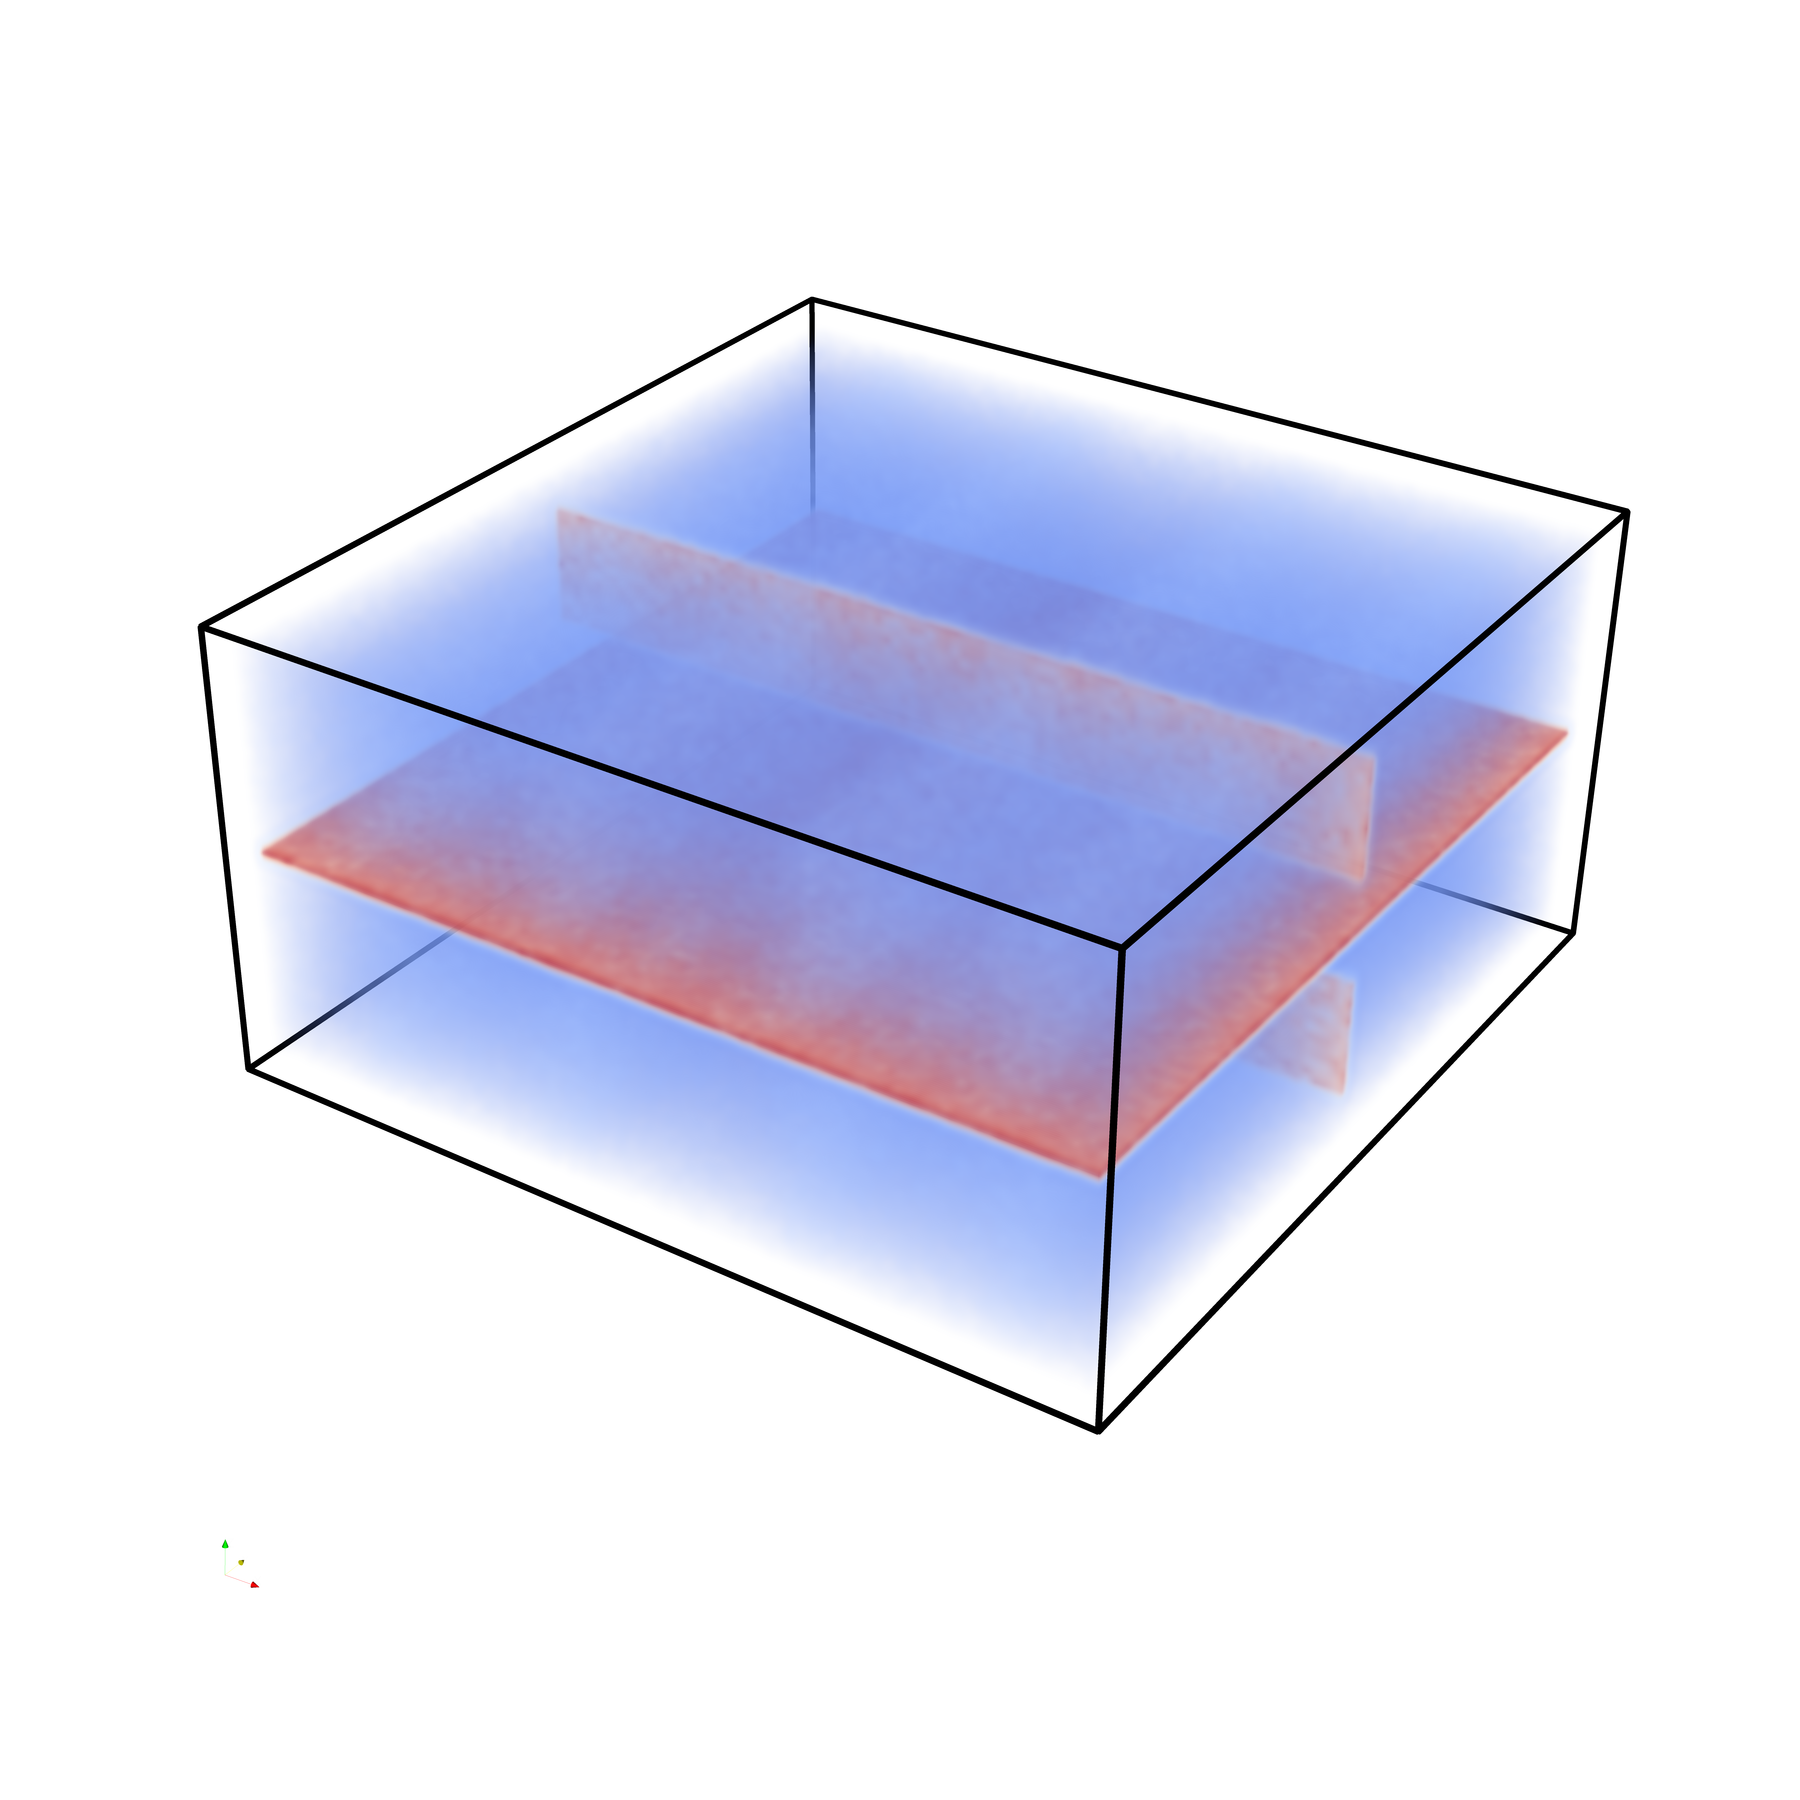
\includegraphics[trim=0 350 0 300, clip=true, width=\textwidth]{Images/shiftXeigen.png}
        \caption{Eigendecomposition}
        \label{fig:shiftXeigen}
    \end{subfigure}
    \begin{subfigure}[b]{0.49\textwidth}
        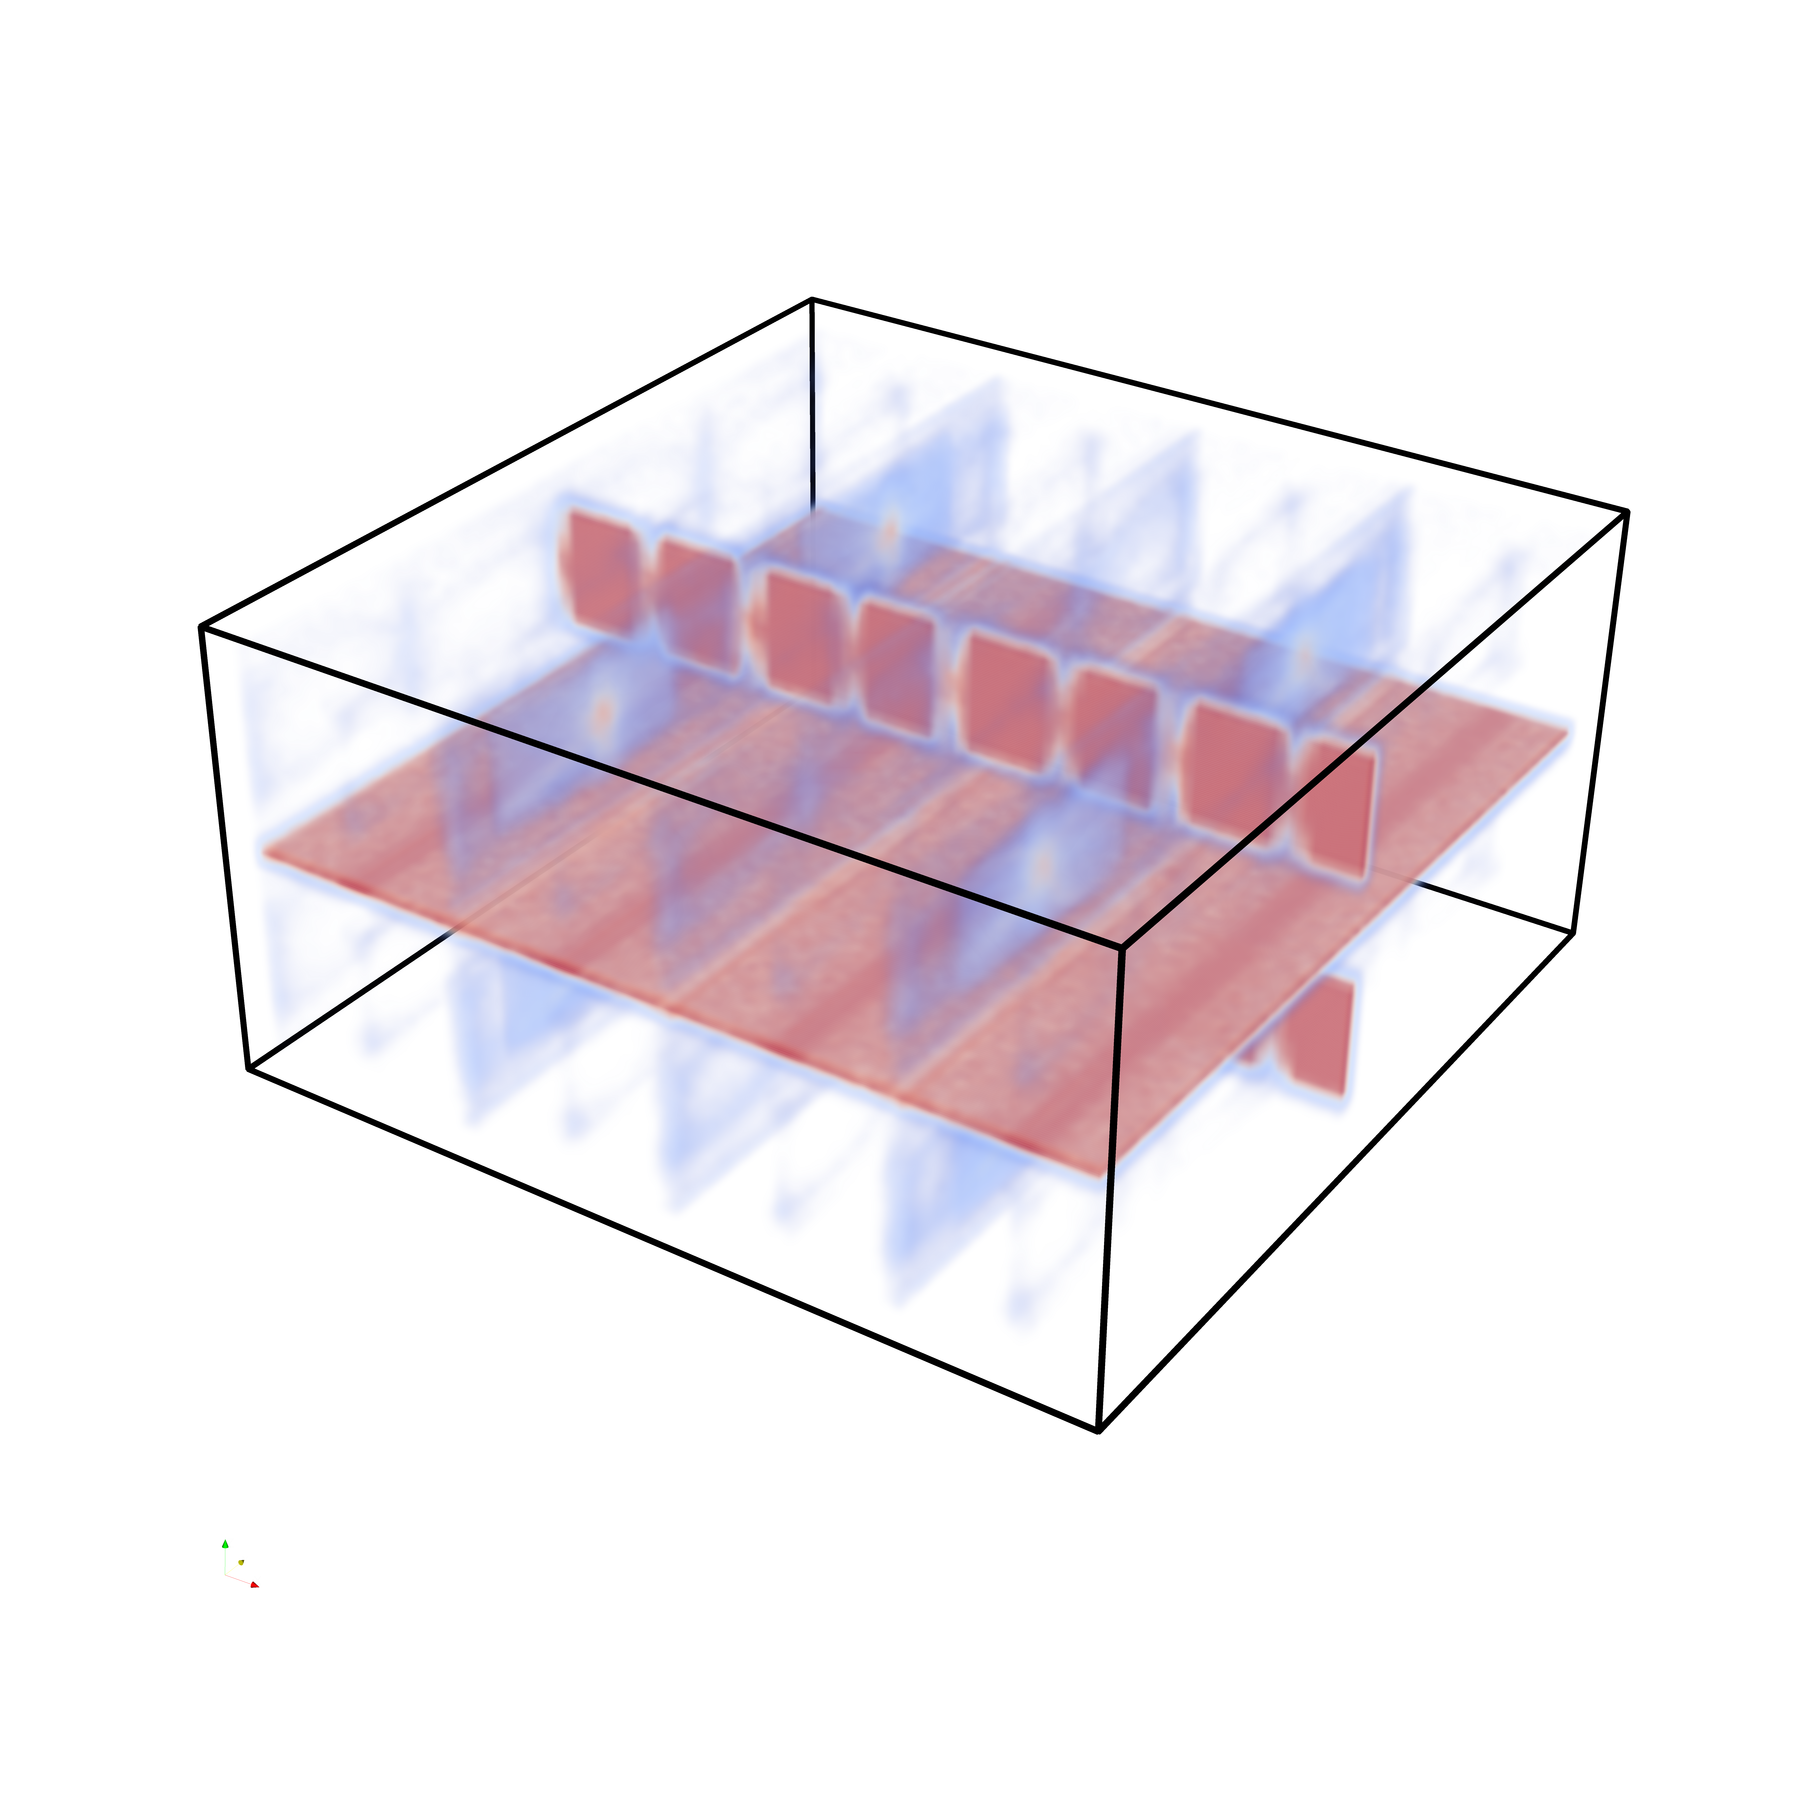
\includegraphics[trim=0 350 0 300, clip=true, width=\textwidth]{Images/shiftXcholesky.png}
        \caption{Cholesky}
        \label{fig:shiftXcholesky}
    \end{subfigure}
    \caption{Comparison of the two matrix decompositions for a set
    of fields shifted equally along the $x$ dimension. The 
    Eigendecomposition gives a smooth estimate of the ridge surface,
    according to the distribution of the ridges in the members.
    Cholesky exhibits lower probabilities at points where the
    ridge should be very certain, due to interferences.}
    \label{fig:decomps}
\end{figure}
\indent To understand what happened here, we will again take a look at
samples drawn from the distribution of Figure~\ref{fig:sampComp}.
Figure~\ref{fig:MDsampComp} shows the gradients of two samples from
either decomposition with their respective unscaled eigenvectors at the
base. Even though the Eigendecomposition in Figure~\ref{fig:sampleEig}
breaks the parallelity of the original field, the gradients still point
in the same general direction and the eigenvectors are consistently
oriented. The gradients of Cholesky on the other hand have no
directional correlation at all. The direction of the vectors is
arbitrary along the distribution and therefore their eigenvectors
have inconsistent orienting as well. The Eigendecomposition seems
to keep the correlation of elements of individual members, whereas
Cholesky mingles the members in one sample. For the calculation of
a ridge feature which depends on precision, this is an issue.\\
\begin{figure}
    \begin{subfigure}[b]{0.49\textwidth}
        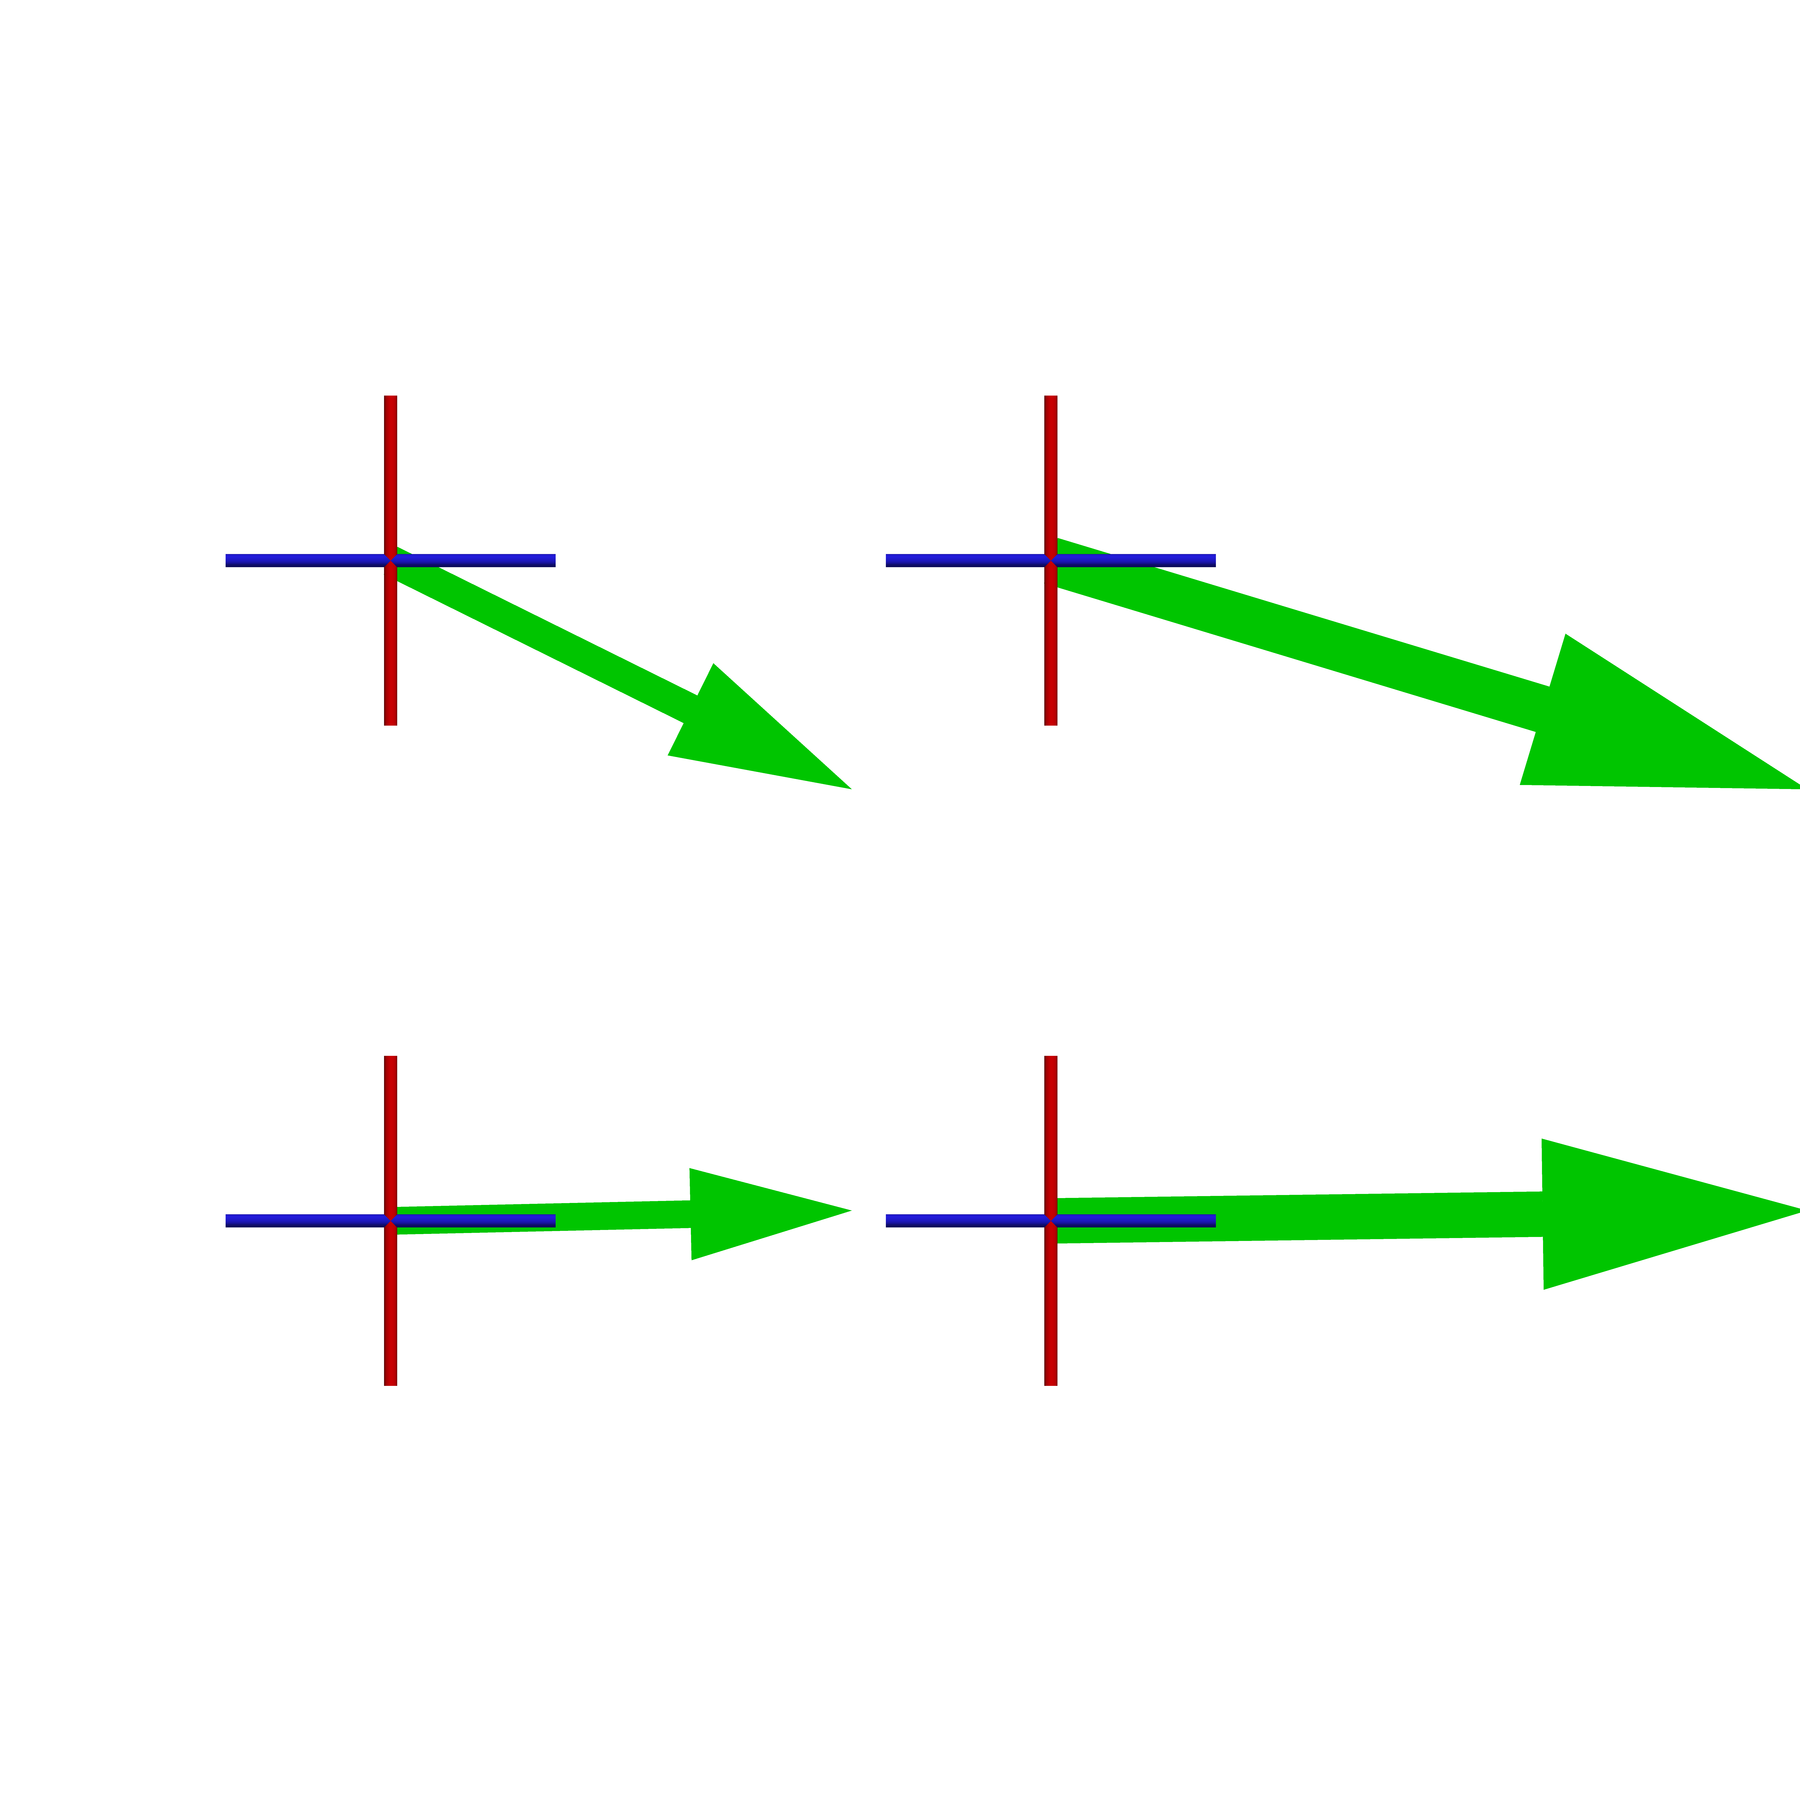
\includegraphics[trim=0 350 0 100, clip=true, width=\textwidth]{Images/sampleEig.png}
        \caption{Eigendecomposition}
        \label{fig:sampleEig}
    \end{subfigure}
    \centering
    \begin{subfigure}[b]{0.49\textwidth}
        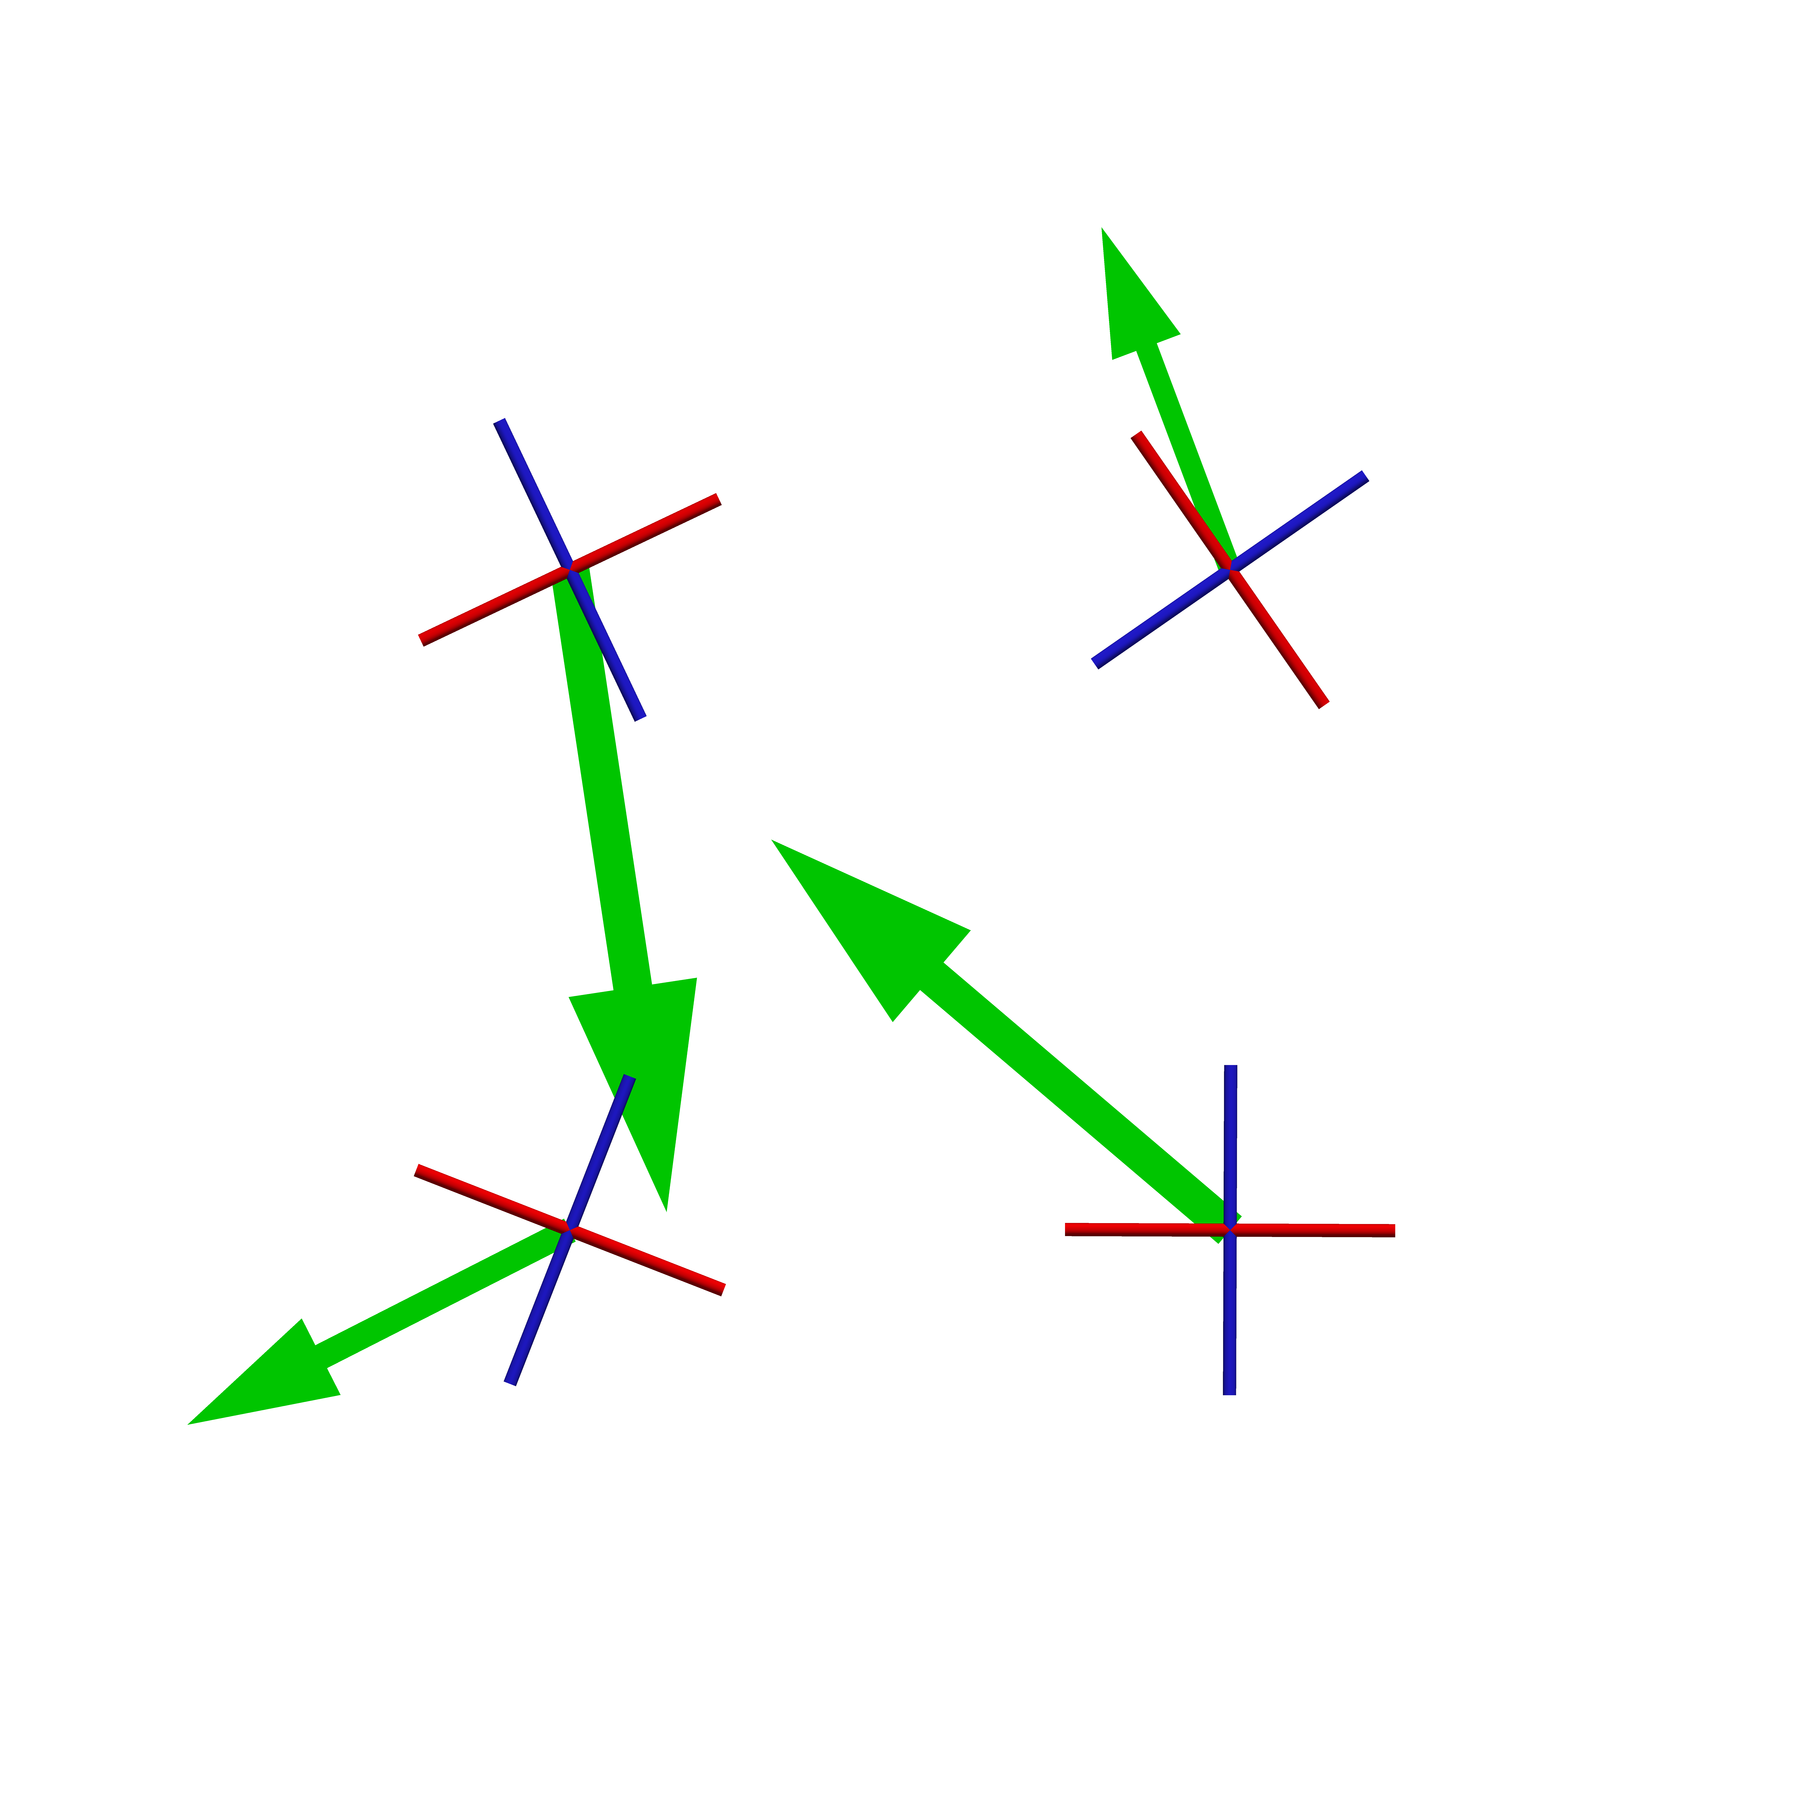
\includegraphics[trim=0 350 0 100, clip=true, width=\textwidth]{Images/sampleChol.png}
        \caption{Cholesky}
        \label{fig:sampleChol}
    \end{subfigure}
    \caption{Gradients of samples from the distribution of the rotated
    field for $f(x,y)=x^2$. The samples from the Eigendecomposition
    keep the structure of the original fields, whereas the Cholesky
    decomposition mixes the distributions in one sample.}
    \label{fig:MDsampComp}
\end{figure}
\indent The differences are the consequence of the immanent nature of the
decompositions. The Eigendecomposition of the covariance matrix
equals to the Principal Component Analysis and therefore the scaled
eigenvectors equal to the uncertainty of $\Sigma$ along
the direction of the eigenvector. If we now multiply a standard normal
distributed vector $N$ with $A = E\Lambda$, every $i$-th component of
$N$ is multiplied with a component of the $i$-th column of $A$, and thus
the $i$-th eigenvector. This leads to a constant scaling of elements
along the direction of an eigenvectors. Cholesky produces a lower
triangular matrix for $A=LD^{\frac{1}{2}}$, thus the columns have
increasing influence on the distribution of the sample with increasing
$i$, but the first element of the sample vector is only determined by
the scaling of $a_{11}$ with the random number at $N_1$. An interesting
implementation detail is, that the algorithm calculating the eigenvalues
for our large covariance matrices uses the power iteration method, that
estimates the largest absolute eigenvalue $\lambda$ in $\mathcal{O}
(N^2)$. Then the matrix is reduced by $A-\lambda I$ and power iteration
is applied again. This process can be repeated until all eigenvalues are
found. Analytic results are too computationally intensive for matrices
of size $80 \times 80$ or $24 \times 24$. Due to this algorithm, the
first column of our eigenvectormatrix always corresponds to the largest
eigenvalue, and therefore the axis with the greatest variance of the
set. Comparing this to the Cholesky decomposition, we could say that the
samples from Cholesky are mainly influenced by one axis of variance of
the data set, and decreasingly influenced by the latter variances,
resulting in more random samples.\\
\indent Ond\v{r}ej Straka \etal{\cite{MD}} studied the different matrix
decompositions in the context of Unscented Kalman Filters, but their
results are applicable for our case as well. They drew three conclusions
after their analysis of the decompositions: If the variable we want to
sample contains no correlated elements, the samples for both
decompositions are equally good and therefore the Cholesky decomposition
might be prefered because of its faster computation time. If the
variable contains correlated elements, the choice may significantly
affect the quality of the sample and, if the elements exhibit strong
correlation, numerical stability becomes an issue as well, especially
for Cholesky, as the covariance matrix with strong correlation becomes
nearly singular. Considering, that we usually apply the uncertain ridge
extraction to data sets obtained from simulations, we will have strong
correlation of the members of the data set for the most parts of the
field. The difference of the decompositions is particularly visible when
comparing the results obtained from the ridge extraction using Marching
Cubes (Figure~\ref{fig:MCcomp}). Cholesky produces the same structure as
in Figure~\ref{fig:shiftXcholesky}, but with more certainty. This is a
misleading representation of the underlying uncertainty. The results
obtained from the Eigendecomposition (Figure~\ref{fig:MCeigen}) on the
other hand can almost be considered better than the ones with our new
criterion, as the high probabilities are notably thinner distributed,
just like the certain ridge would be. We will compare the two approaches
in the next section.\\
\indent Concluding from all of this, the Eigendecomposition delivers
better results in most cases. Only if we have strong uncertainty in the
data, the Cholesky decomposition may give us better results. We took the
set from Figure~\ref{fig:MCridges} and extended it with members having
greater variance along either axis. The results of the two
decompositions can be seen in Figure~\ref{fig:HUCcomp}. The
Eigendecomposition only deliveres weak probabilities for a ridge
structure, hardly distinguishable from the surrounding noise. Here
Cholesky gives us higher probabilities for nodes close to the mean of
the ridges and, because of our criterion, not much clutter. Due to the
high variance of the data set, the members seem to lose their
correlation. The downside is, that this case is not the usual thing for
real world data, where we try to extract ridge structures from similar
scalar fields. 

\begin{figure}[t]
    \begin{subfigure}[b]{0.49\textwidth}
        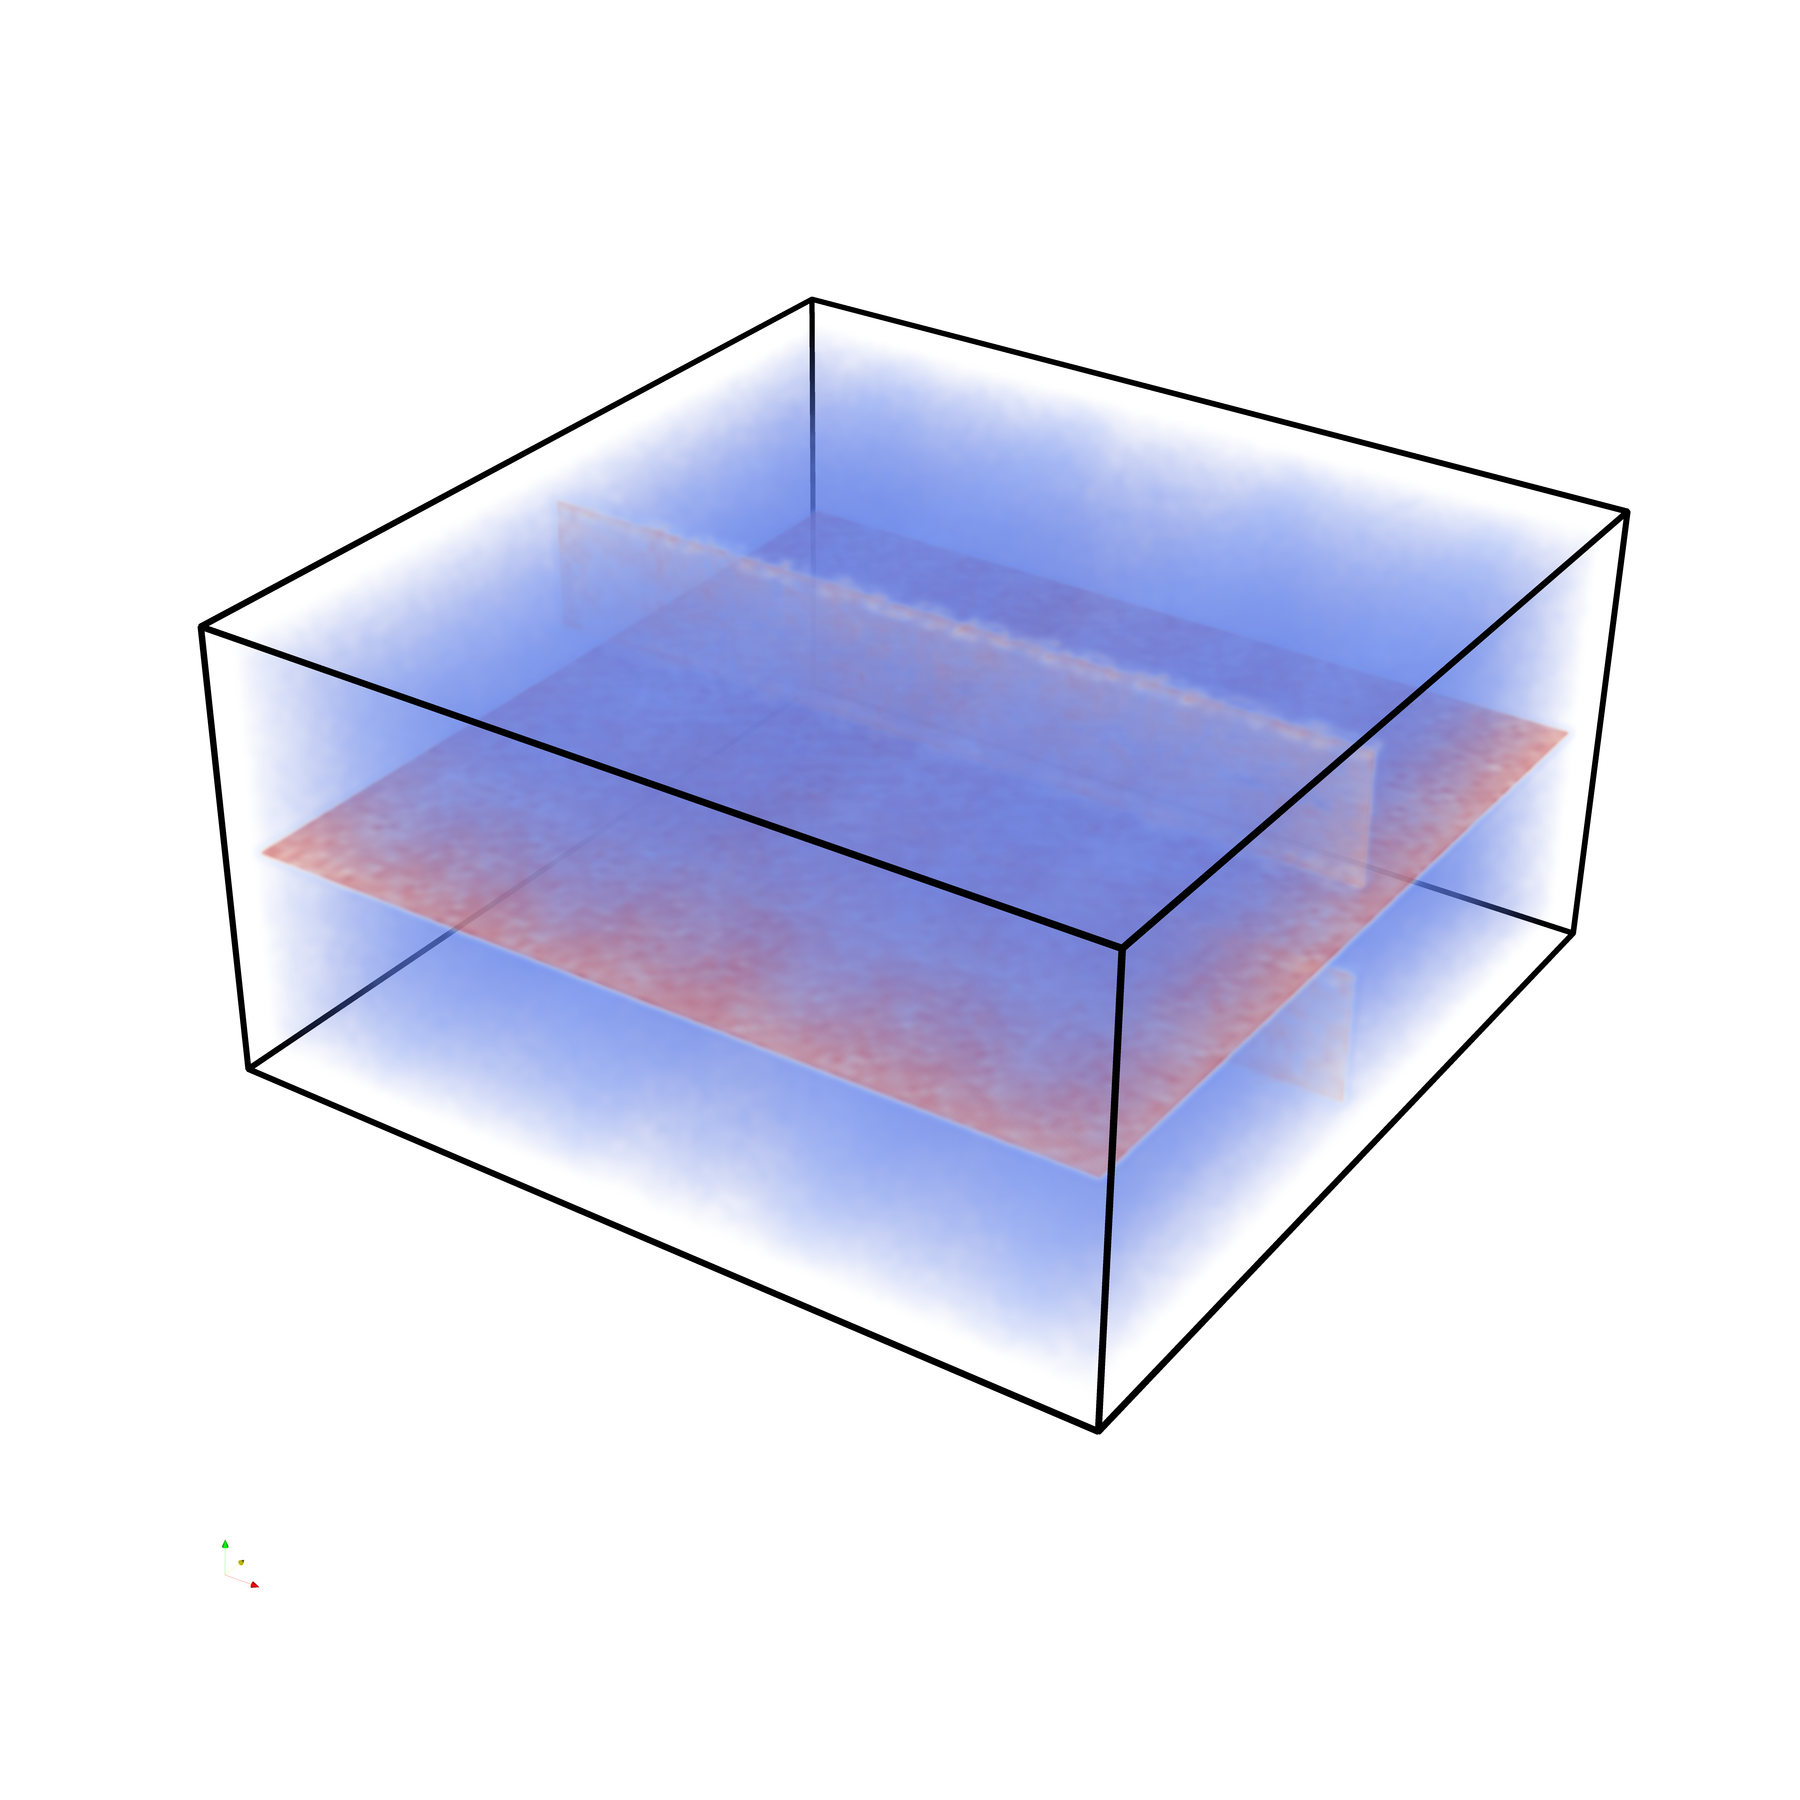
\includegraphics[trim=0 350 0 300, clip=true, width=\textwidth]{Images/shiftXold.png}
        \caption{Eigendecomposition}
        \label{fig:MCeigen}
    \end{subfigure}
    \begin{subfigure}[b]{0.49\textwidth}
        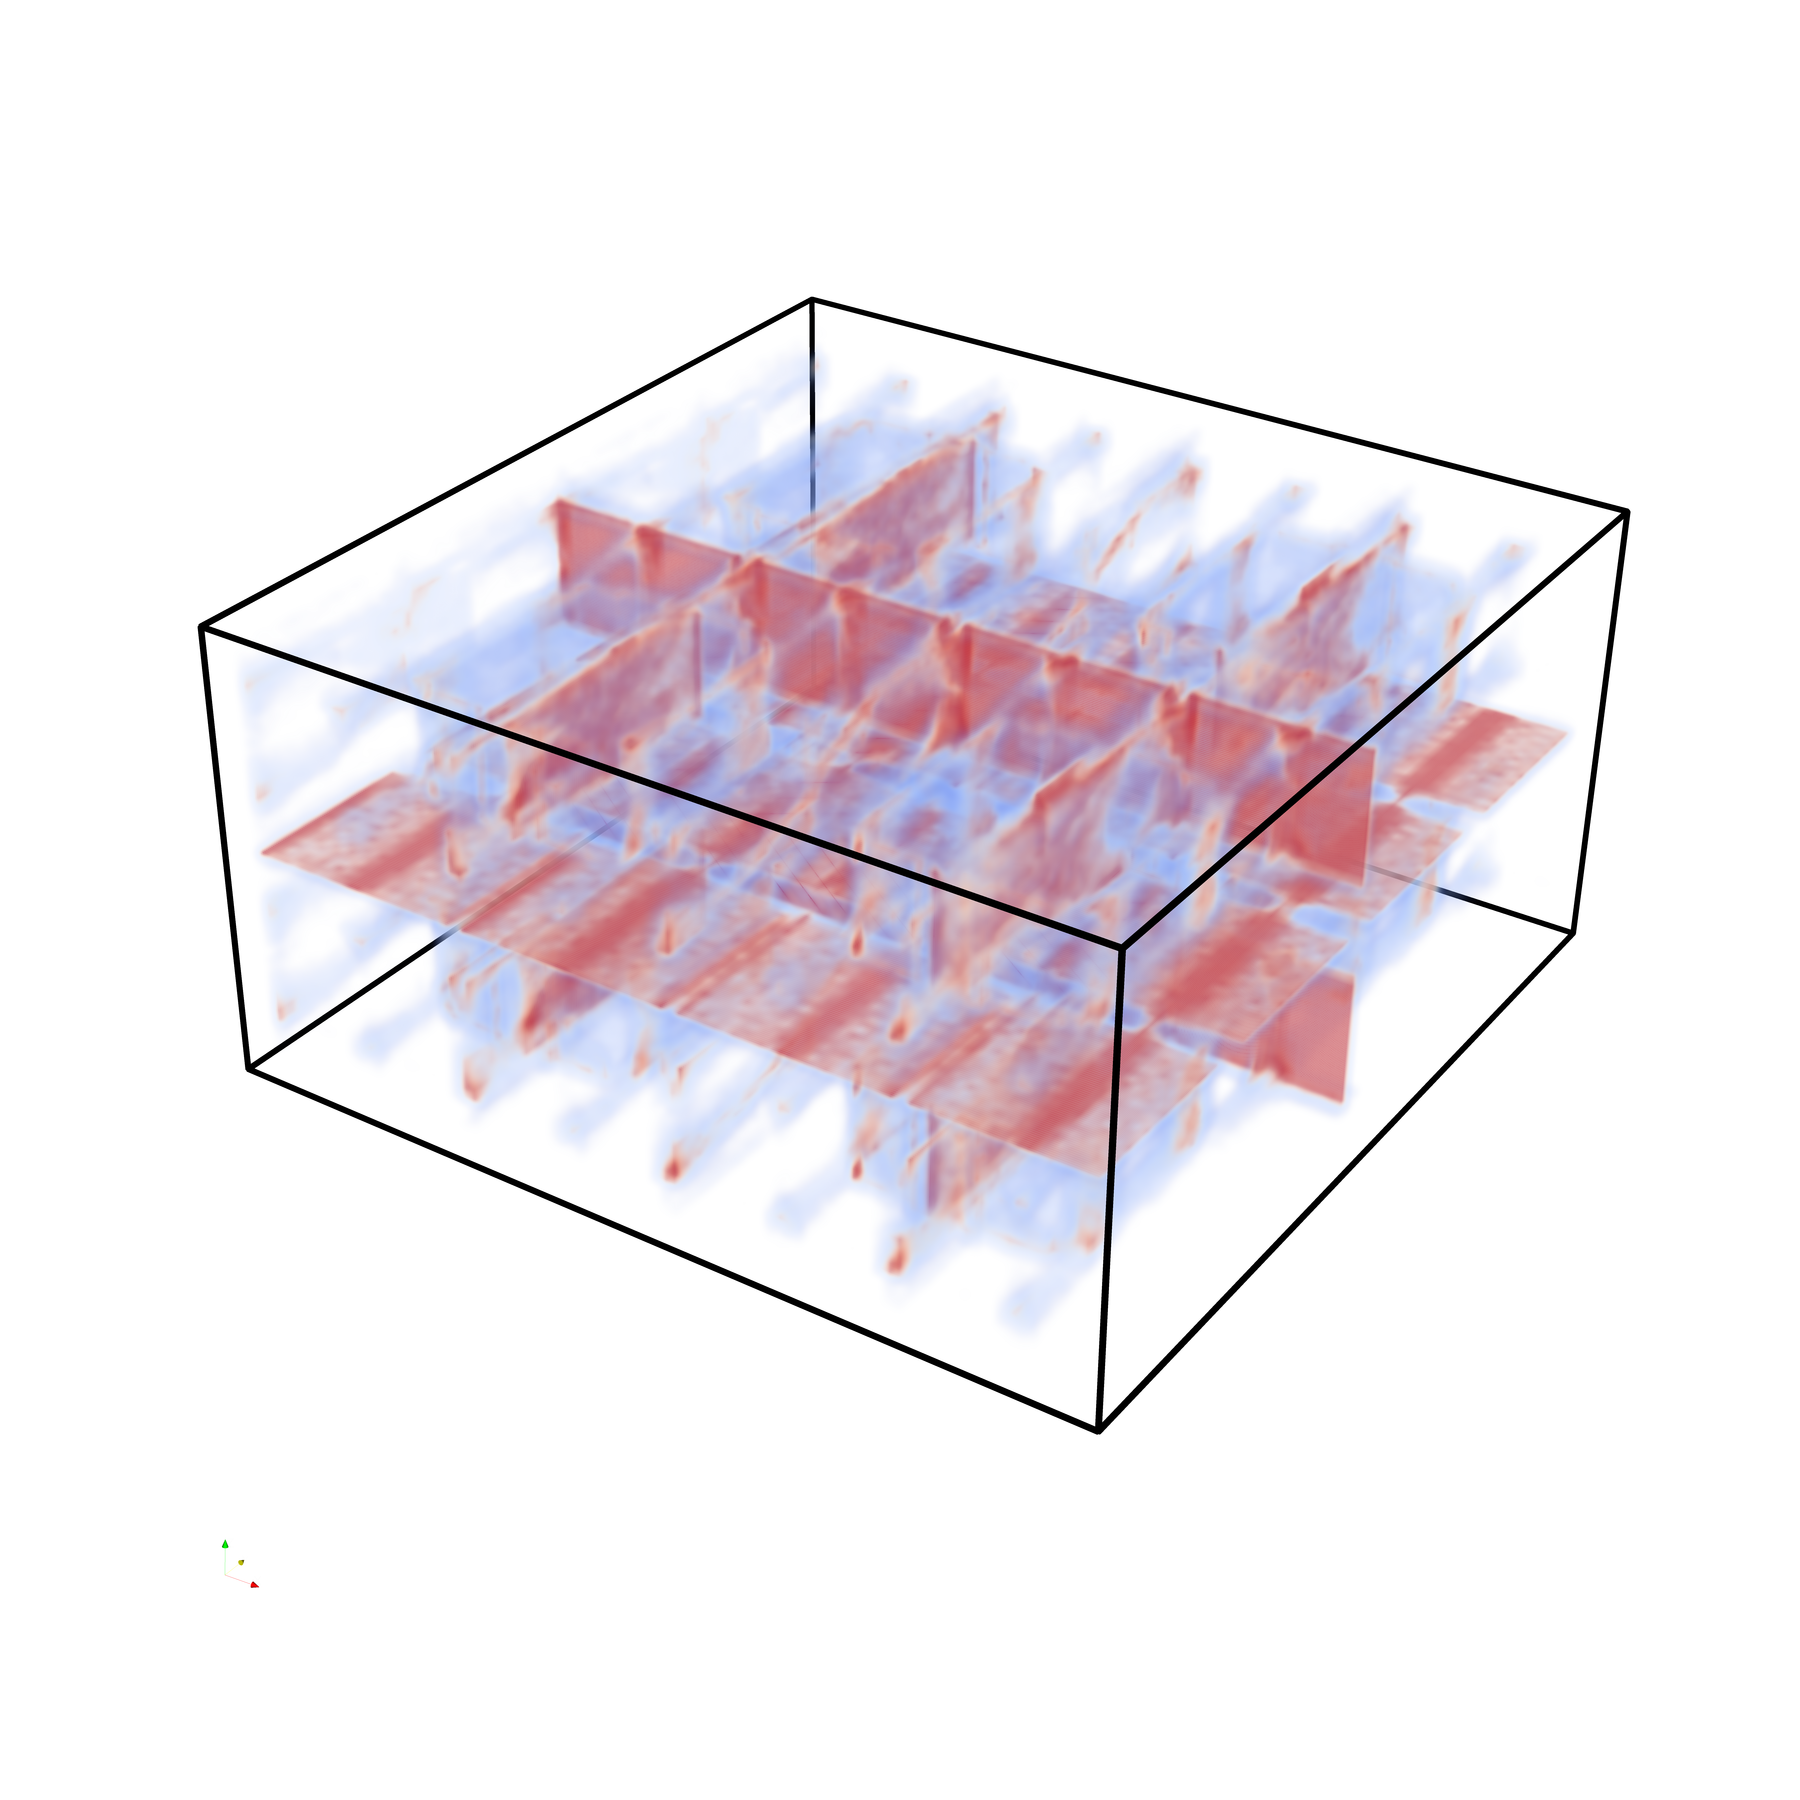
\includegraphics[trim=0 350 0 300, clip=true, width=\textwidth]{Images/shiftXoldchol.png}
        \caption{Cholesky}
        \label{fig:MCchol}
    \end{subfigure}
    \caption{Comparison of matrix decompositions for the uncertain
    ridge extraction using the Uncertain Marching Cubes algorithm. Here, the
    differences are very obvious, as UMC is strongly dependent on the relation
    of the vectors.}
    \label{fig:MCcomp}
\end{figure}

\begin{figure}
    \begin{subfigure}[b]{0.49\textwidth}
        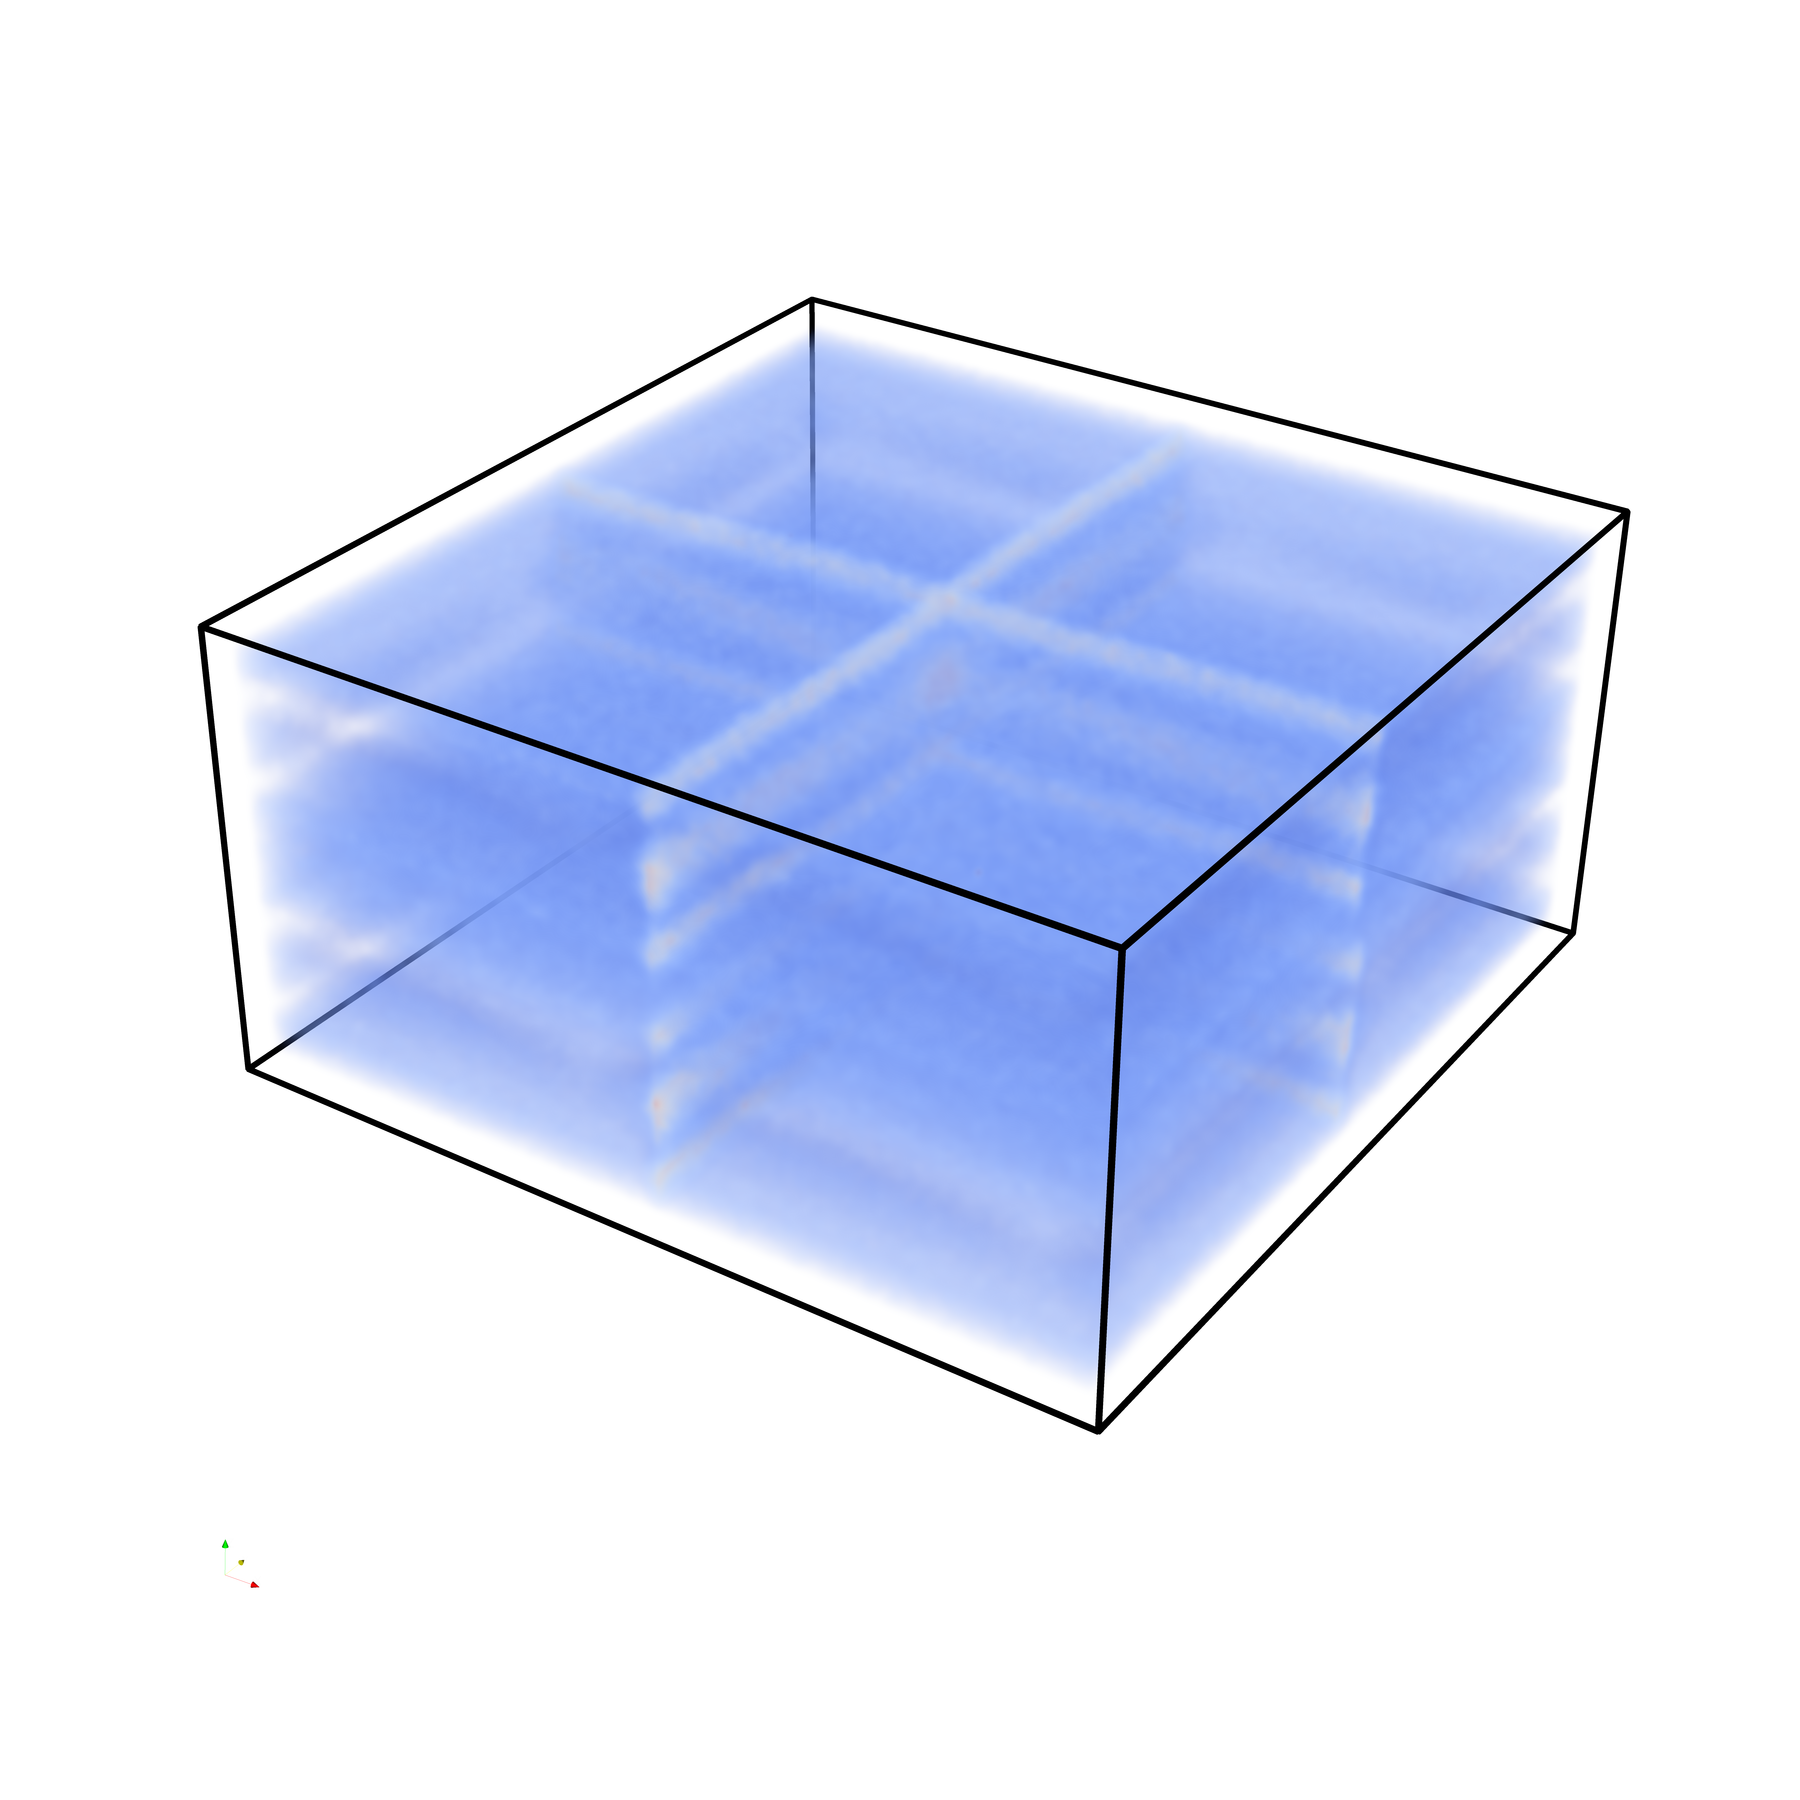
\includegraphics[trim=0 350 0 300, clip=true, width=\textwidth]{Images/highuncEigen.png}
        \caption{Eigendecomposition}
        \label{fig:HUCeigen}
    \end{subfigure}
    \begin{subfigure}[b]{0.49\textwidth}
        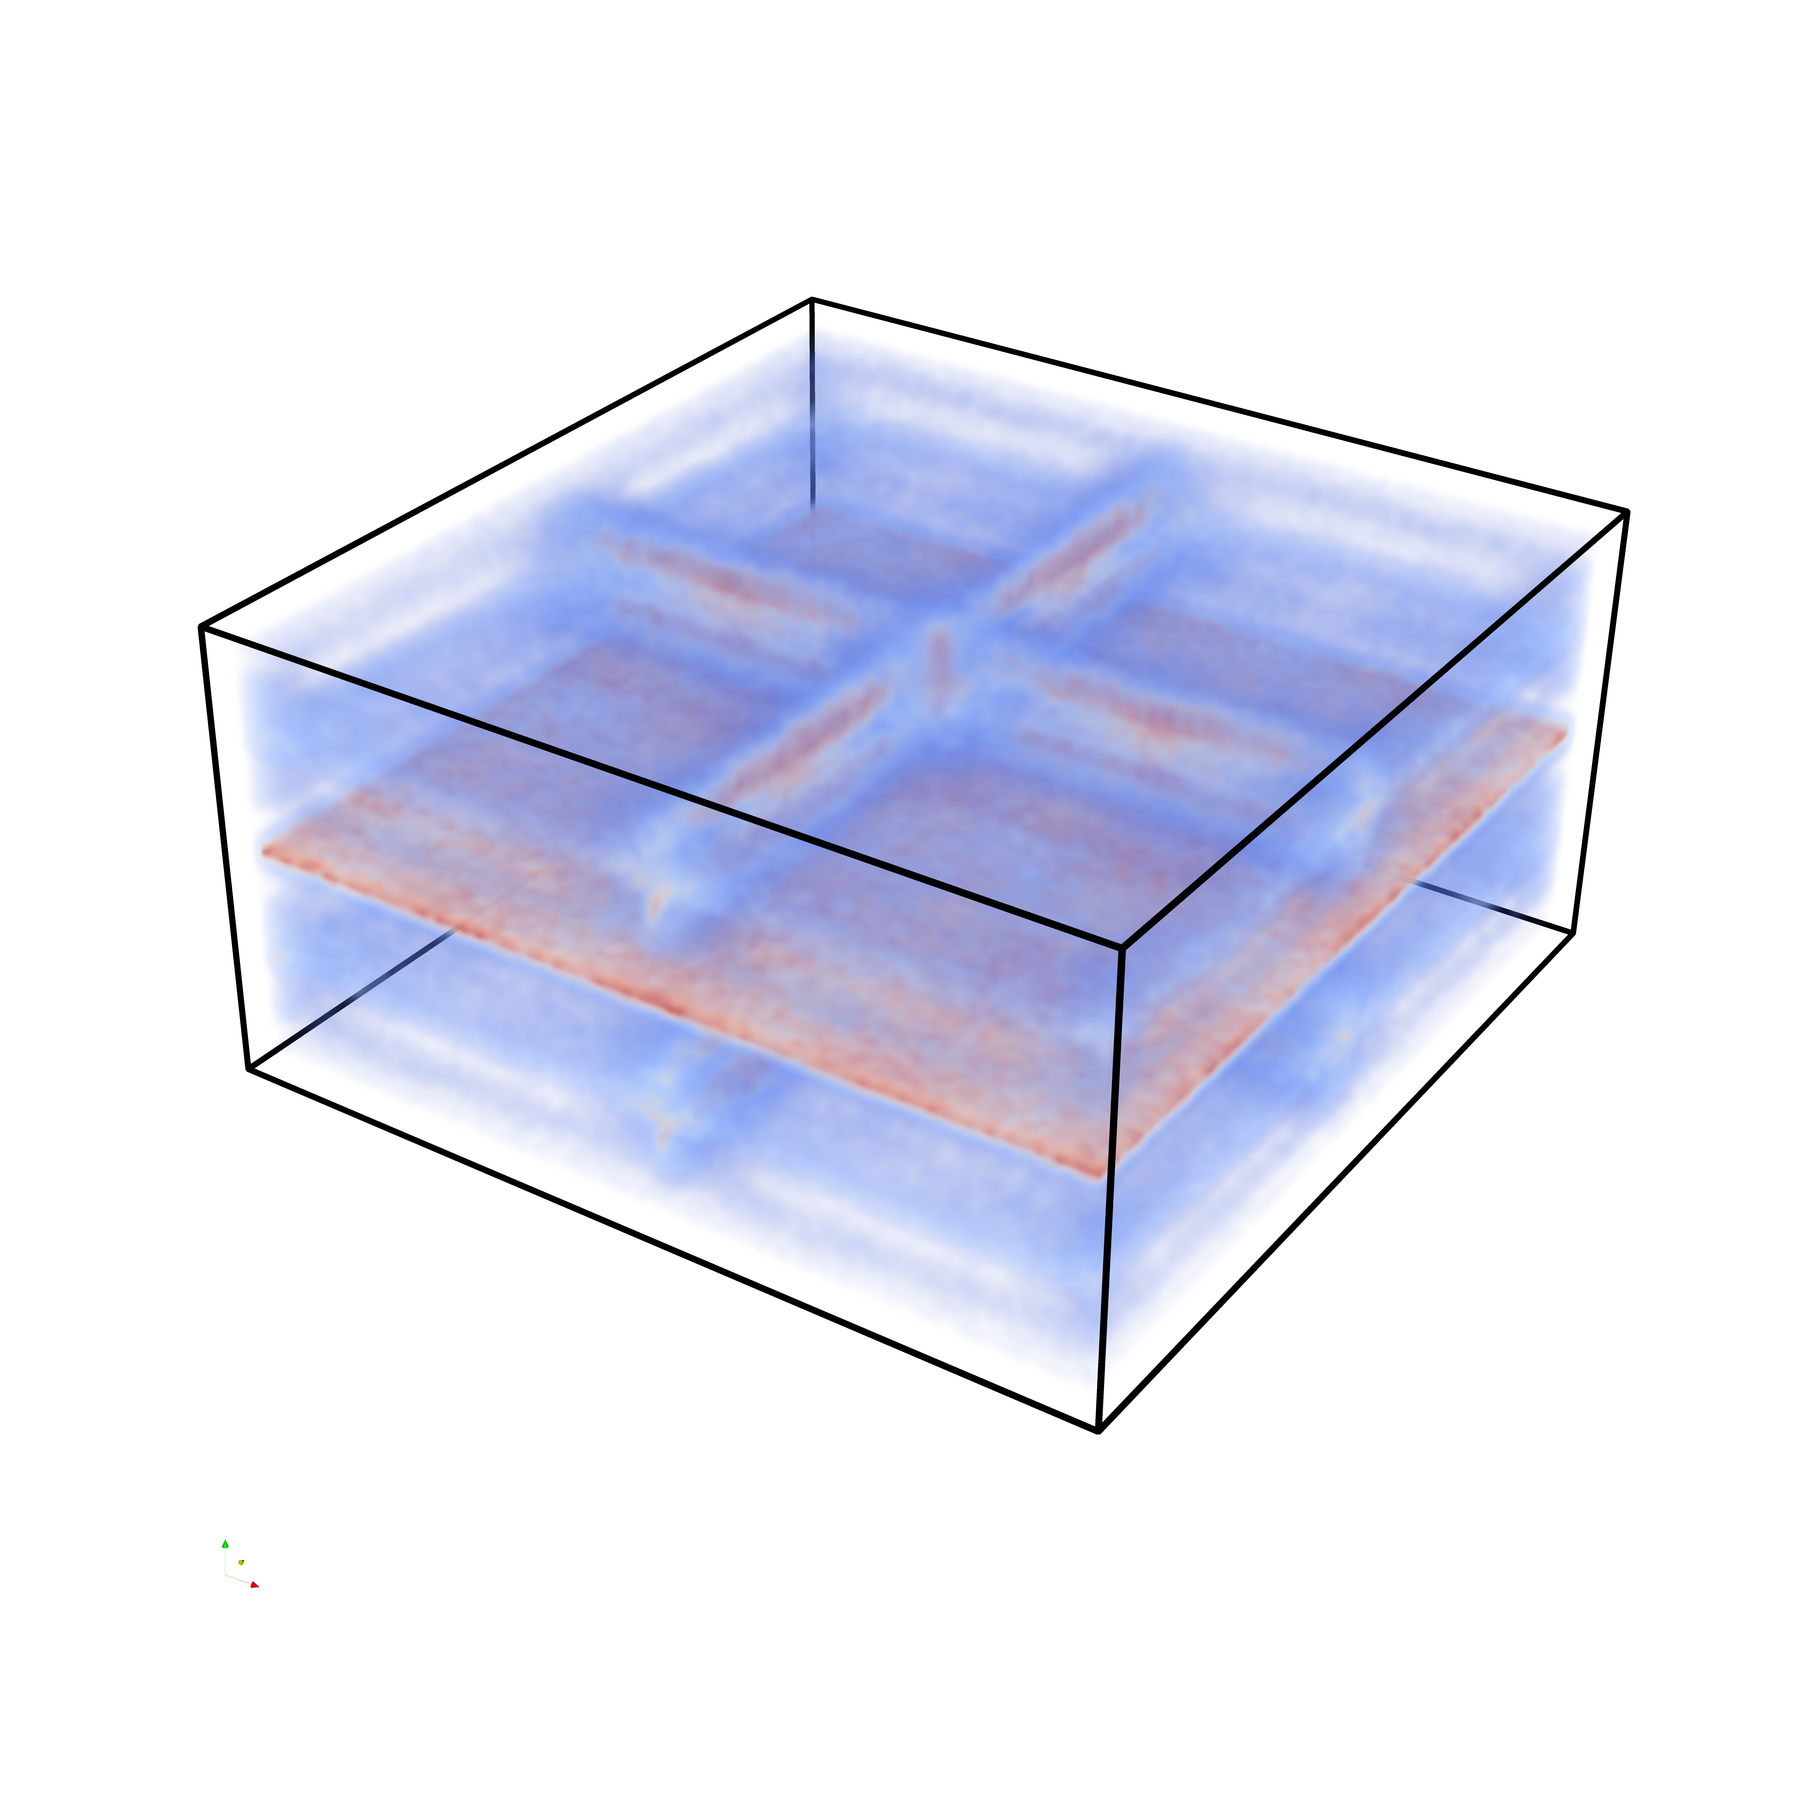
\includegraphics[trim=0 350 0 300, clip=true, width=\textwidth]{Images/highuncChol.png}
        \caption{Cholesky}
        \label{fig:HUCchol}
    \end{subfigure}
    \caption{Comparison of the matrix decompositions for a set with high
    variance in every dimension. The Eigendecomposition exhibits a ridge
    structure appearing roughly around the mean, hardly distinguishable
    from the noise surrounding it. Cholesky delivers a more certain
    structure, with parts missing from the cross like ridges on top and
    bottom, due to the up and downward distortion of the members, but
    still exhibit low probabilities.}
    \label{fig:HUCcomp}
\end{figure}

%%%%%%%%%%%%%%%%%%%%%%%%%%%%%%%%%%%%%%%%%%%%%%%%%%%%%%%%%%%%%%%%%%%%%%%%
\section{Comparison of Extraction Methods}\label{sec:evalExtr}
%%%%%%%%%%%%%%%%%%%%%%%%%%%%%%%%%%%%%%%%%%%%%%%%%%%%%%%%%%%%%%%%%%%%%%%%

After the differences of the decompositions are explained in detail, we
can proceed to evaluate the different approaches for the ridge
extraction. At first we will compare the new criterion to the extraction
with Uncertain Marching Cubes.

%%%%%%%%%%%%%%%%%%%%%%%%%%%%%%%%%%%%%%%%%%%%%%%%%%%%%%%%%%%%%%%%%%%%%%%%
\subsection{Uncertain Marching Cubes or Ridge Estimation}\label{sec:evalMeth}
%%%%%%%%%%%%%%%%%%%%%%%%%%%%%%%%%%%%%%%%%%%%%%%%%%%%%%%%%%%%%%%%%%%%%%%%

\begin{figure}
    \begin{subfigure}{0.49\textwidth}
        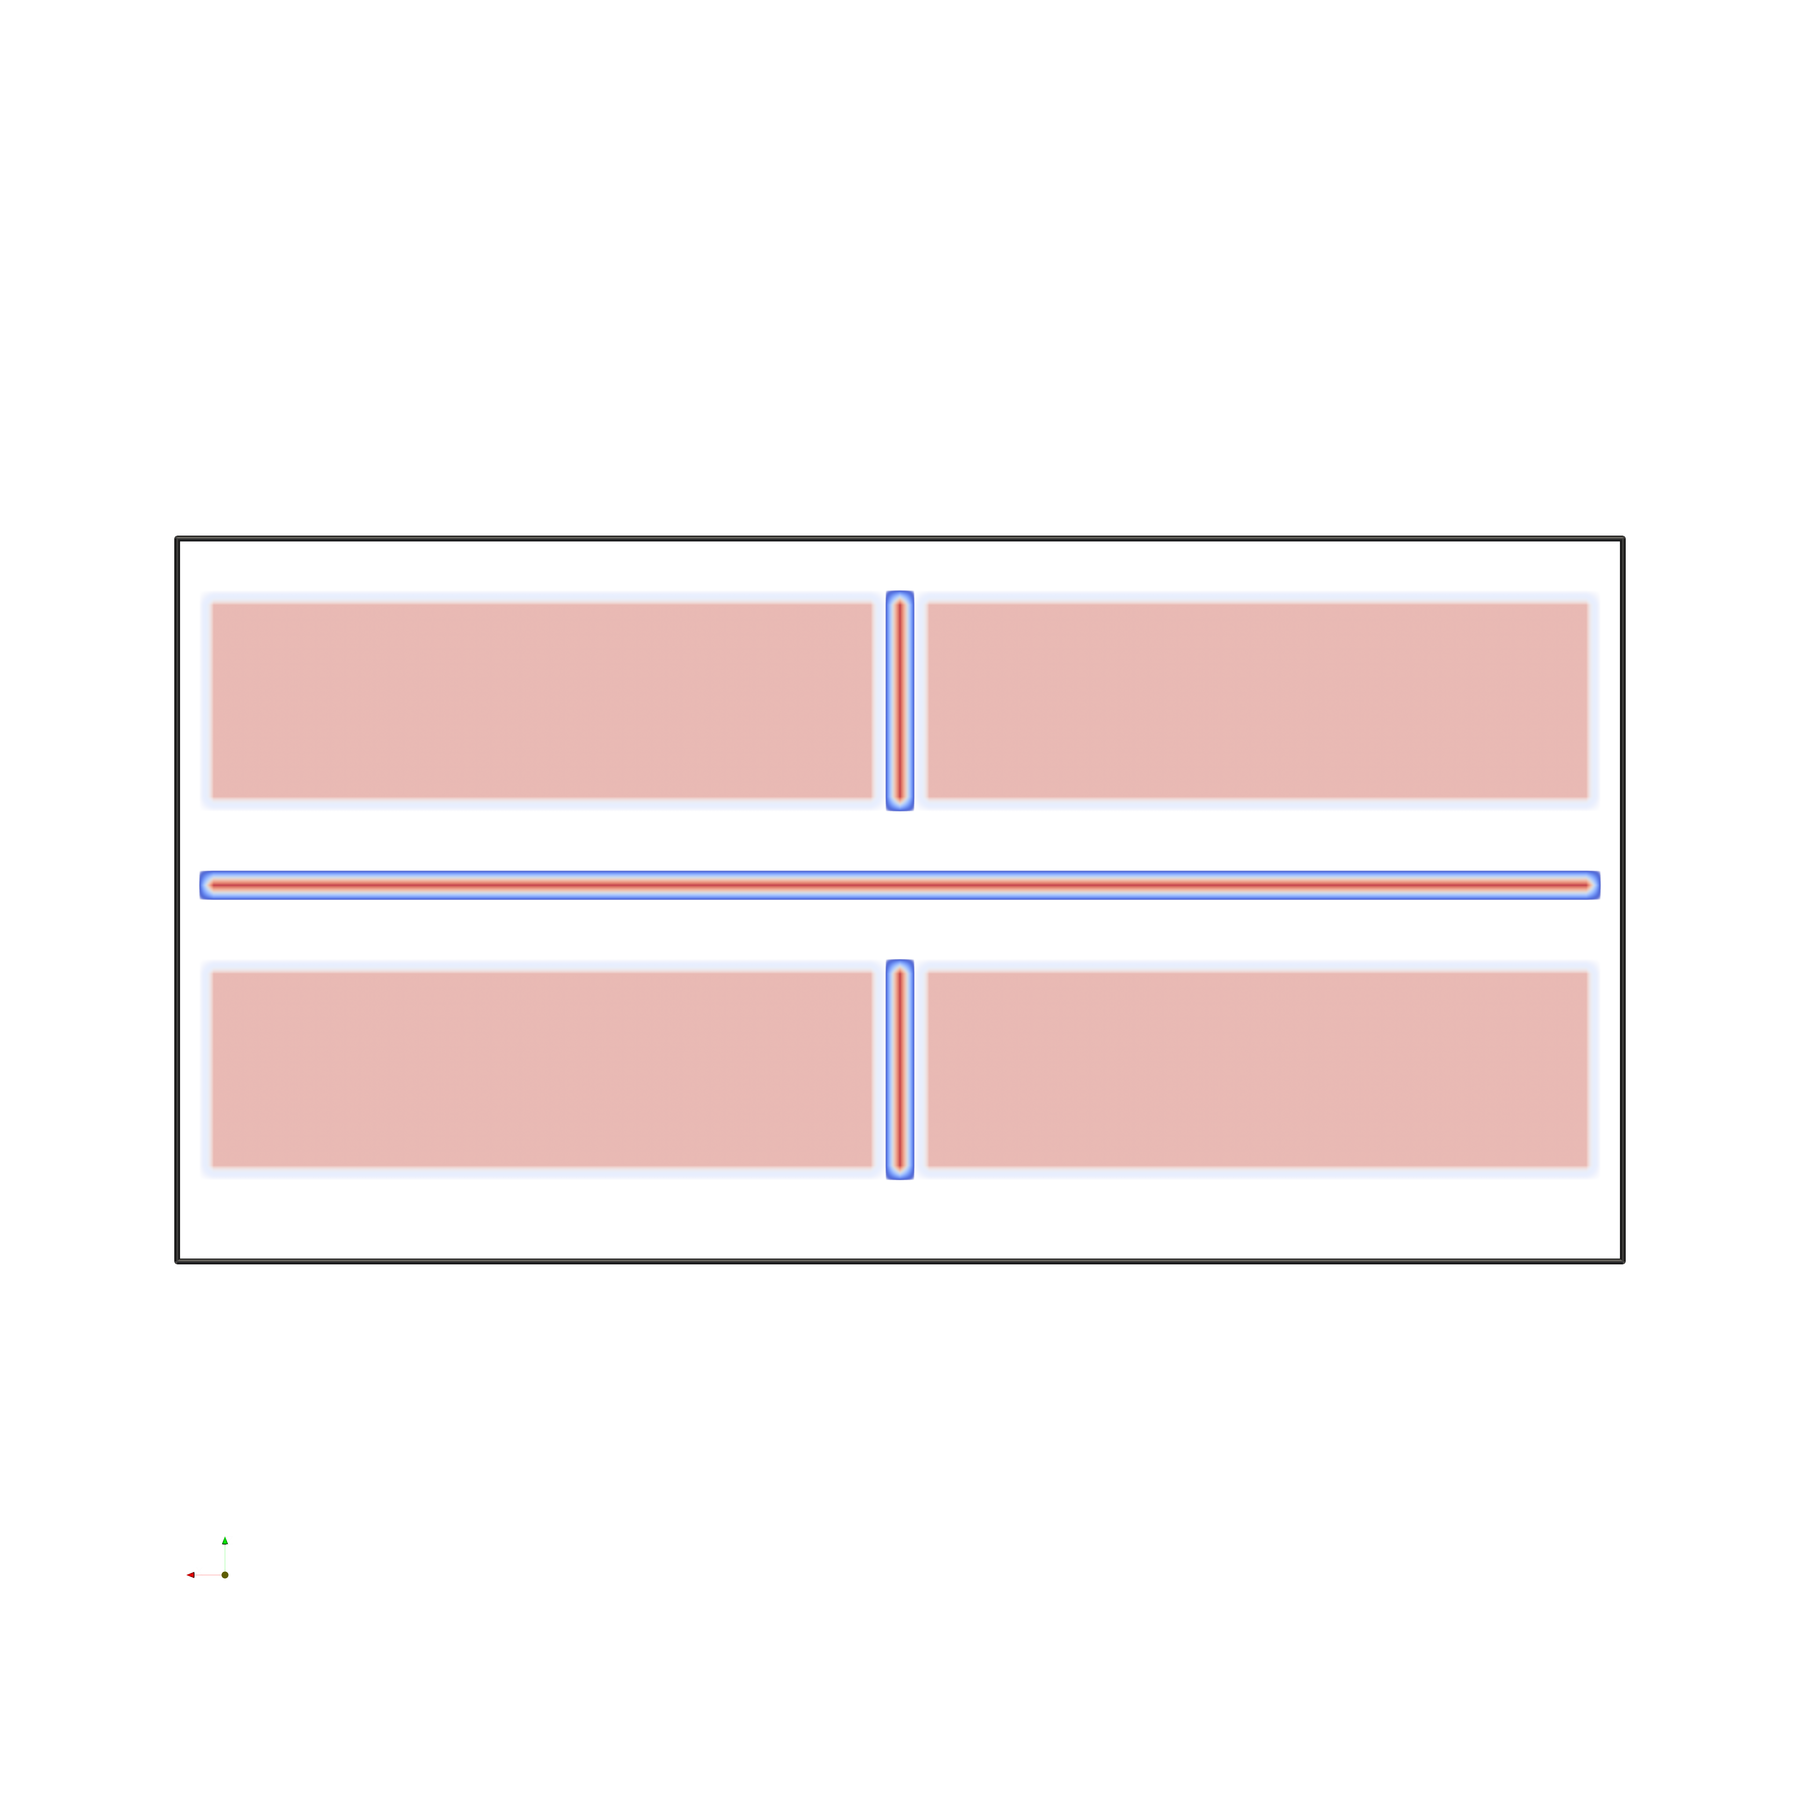
\includegraphics[trim=0 450 0 450, clip=true, width=\textwidth]{Images/oldSide.png}
        \caption{Uncertain Marching Cubes}
        \label{fig:UMCside}
    \end{subfigure}
    \begin{subfigure}{0.49\textwidth}
        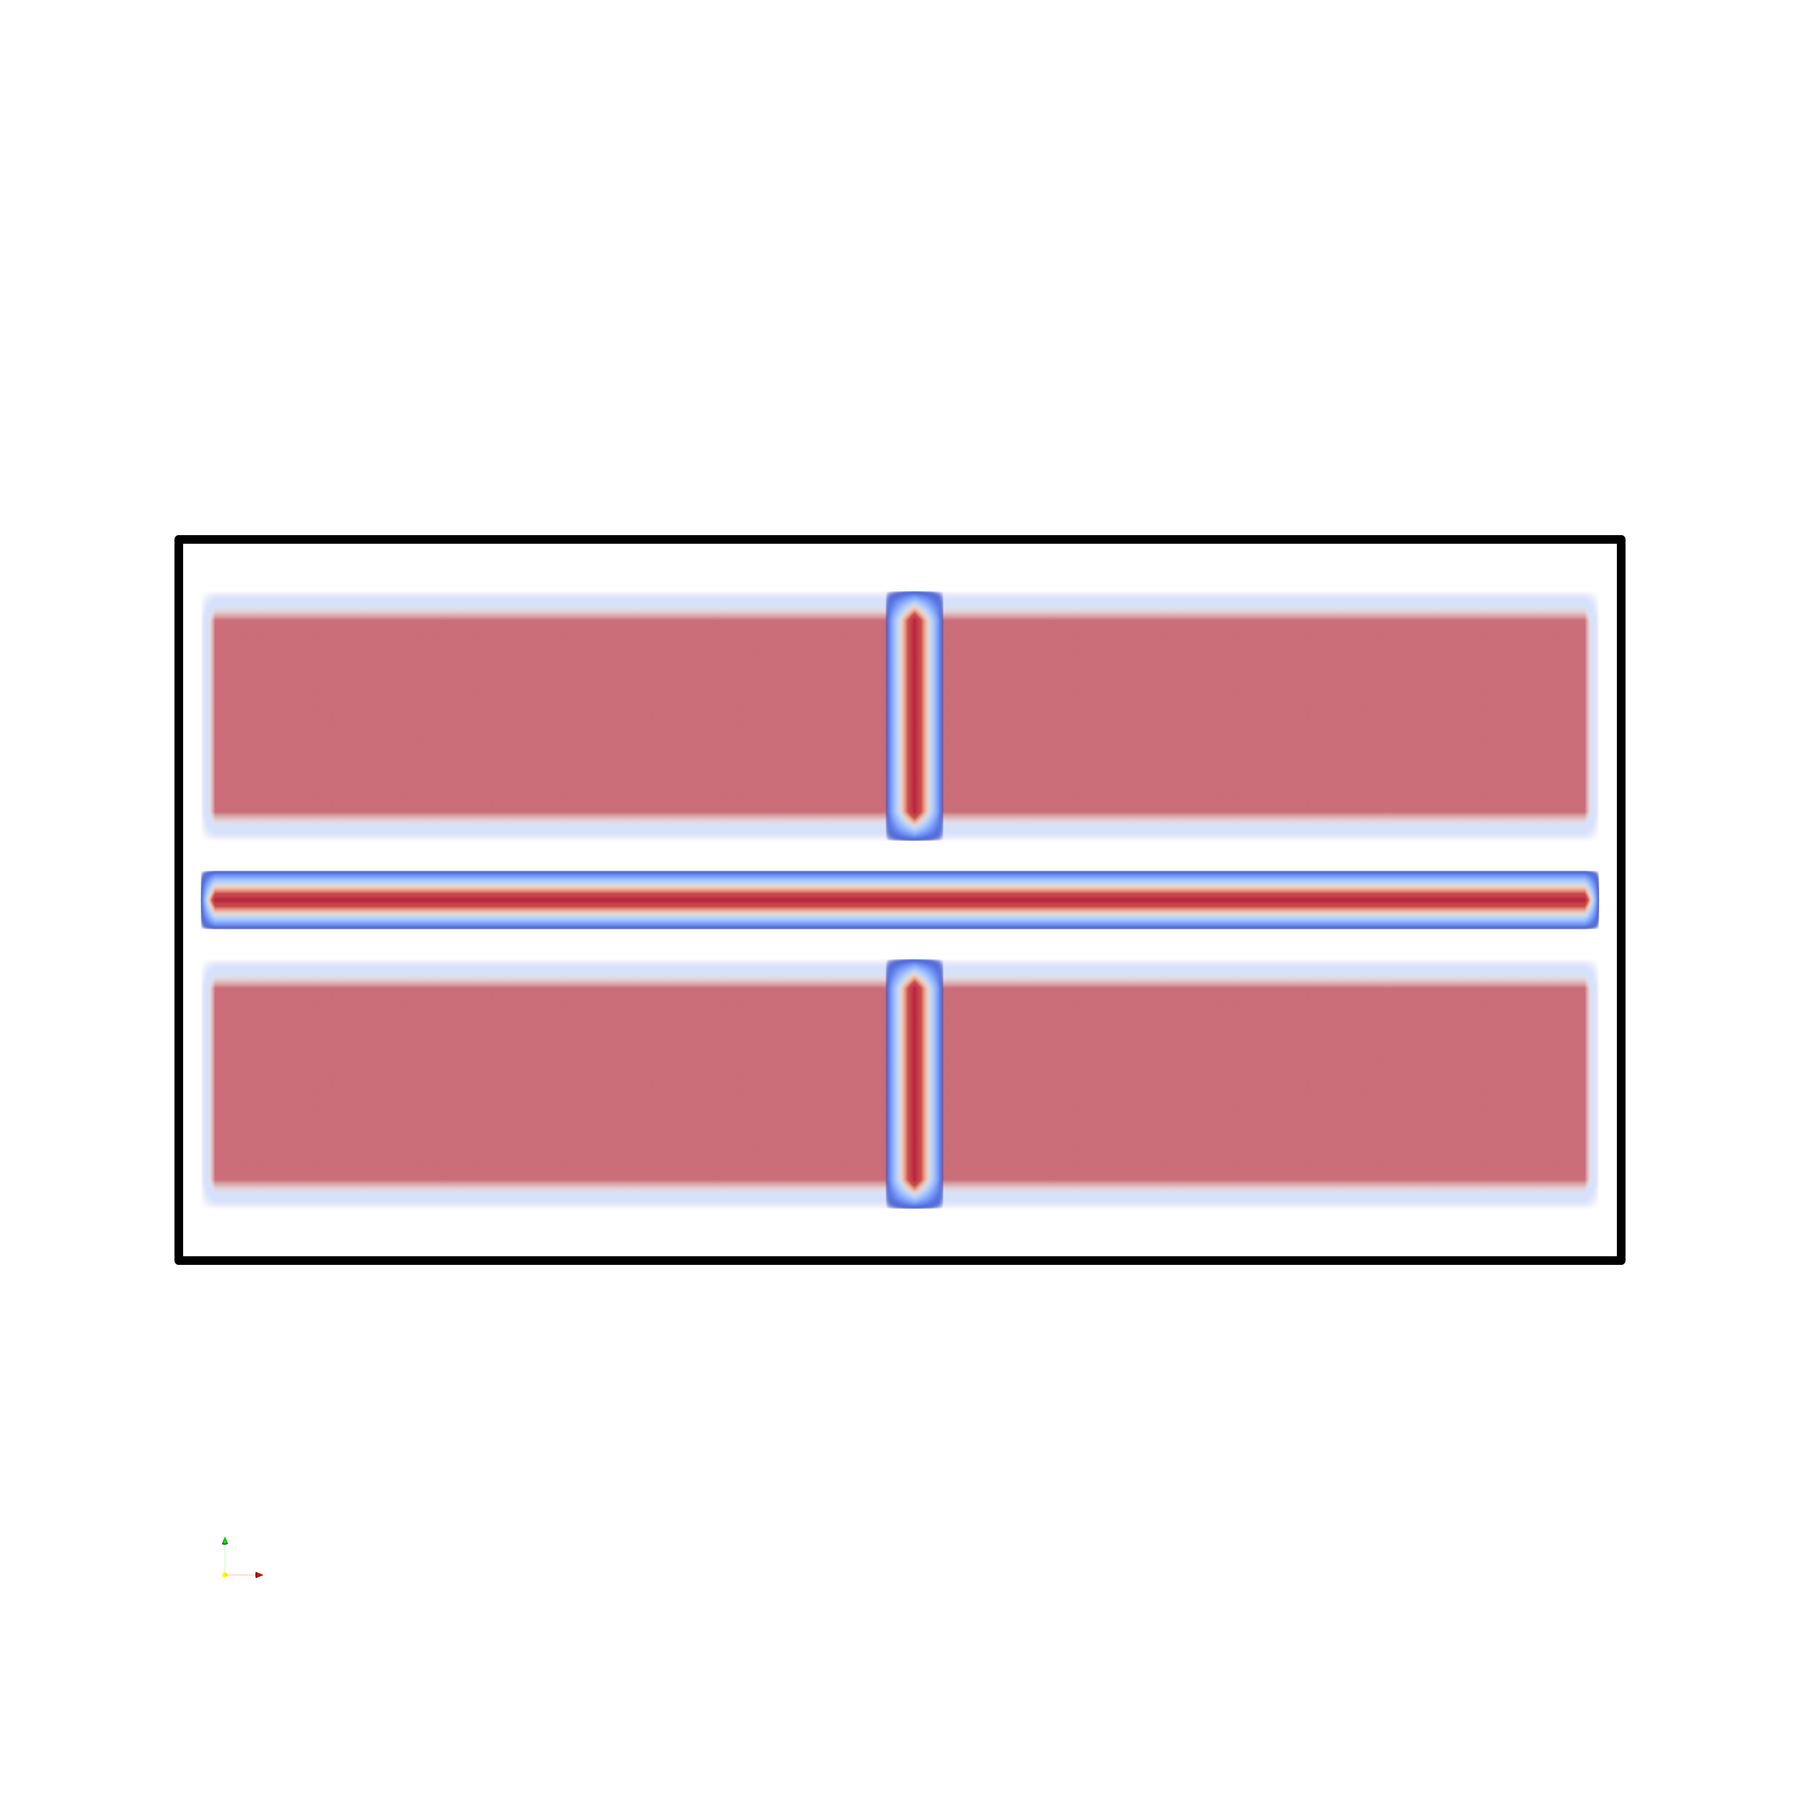
\includegraphics[trim=0 450 0 450, clip=true, width=\textwidth]{Images/newSide.png}
        \caption{Ridge Estimation}
        \label{fig:REside}
    \end{subfigure}
    \caption{Side view of the two extraction methods on a data set with
    no variance. \subref{fig:UMCside} UMC is creating a ridge surface
    with $100\%$ confidence for the thickness of one cell, surrounded by
    another layer of lower probability due to the tolerance for the dot
    product. \subref{fig:REside} Ridge Estimation with the average cell
    distance as $d$, offers a high confidence for 2 to 3 layers of cells
    and still has another layer with lower probability padding it.}
\end{figure}


%%%%%%%%%%%%%%%%%%%%%%%%%%%%%%%%%%%%%%%%%%%%%%%%%%%%%%%%%%%%%%%%%%%%%%%%
\subsection{Ridge Lines in 3D}\label{sec:evalRL}
%%%%%%%%%%%%%%%%%%%%%%%%%%%%%%%%%%%%%%%%%%%%%%%%%%%%%%%%%%%%%%%%%%%%%%%%

\begin{figure}
    \begin{subfigure}{0.33\textwidth}
        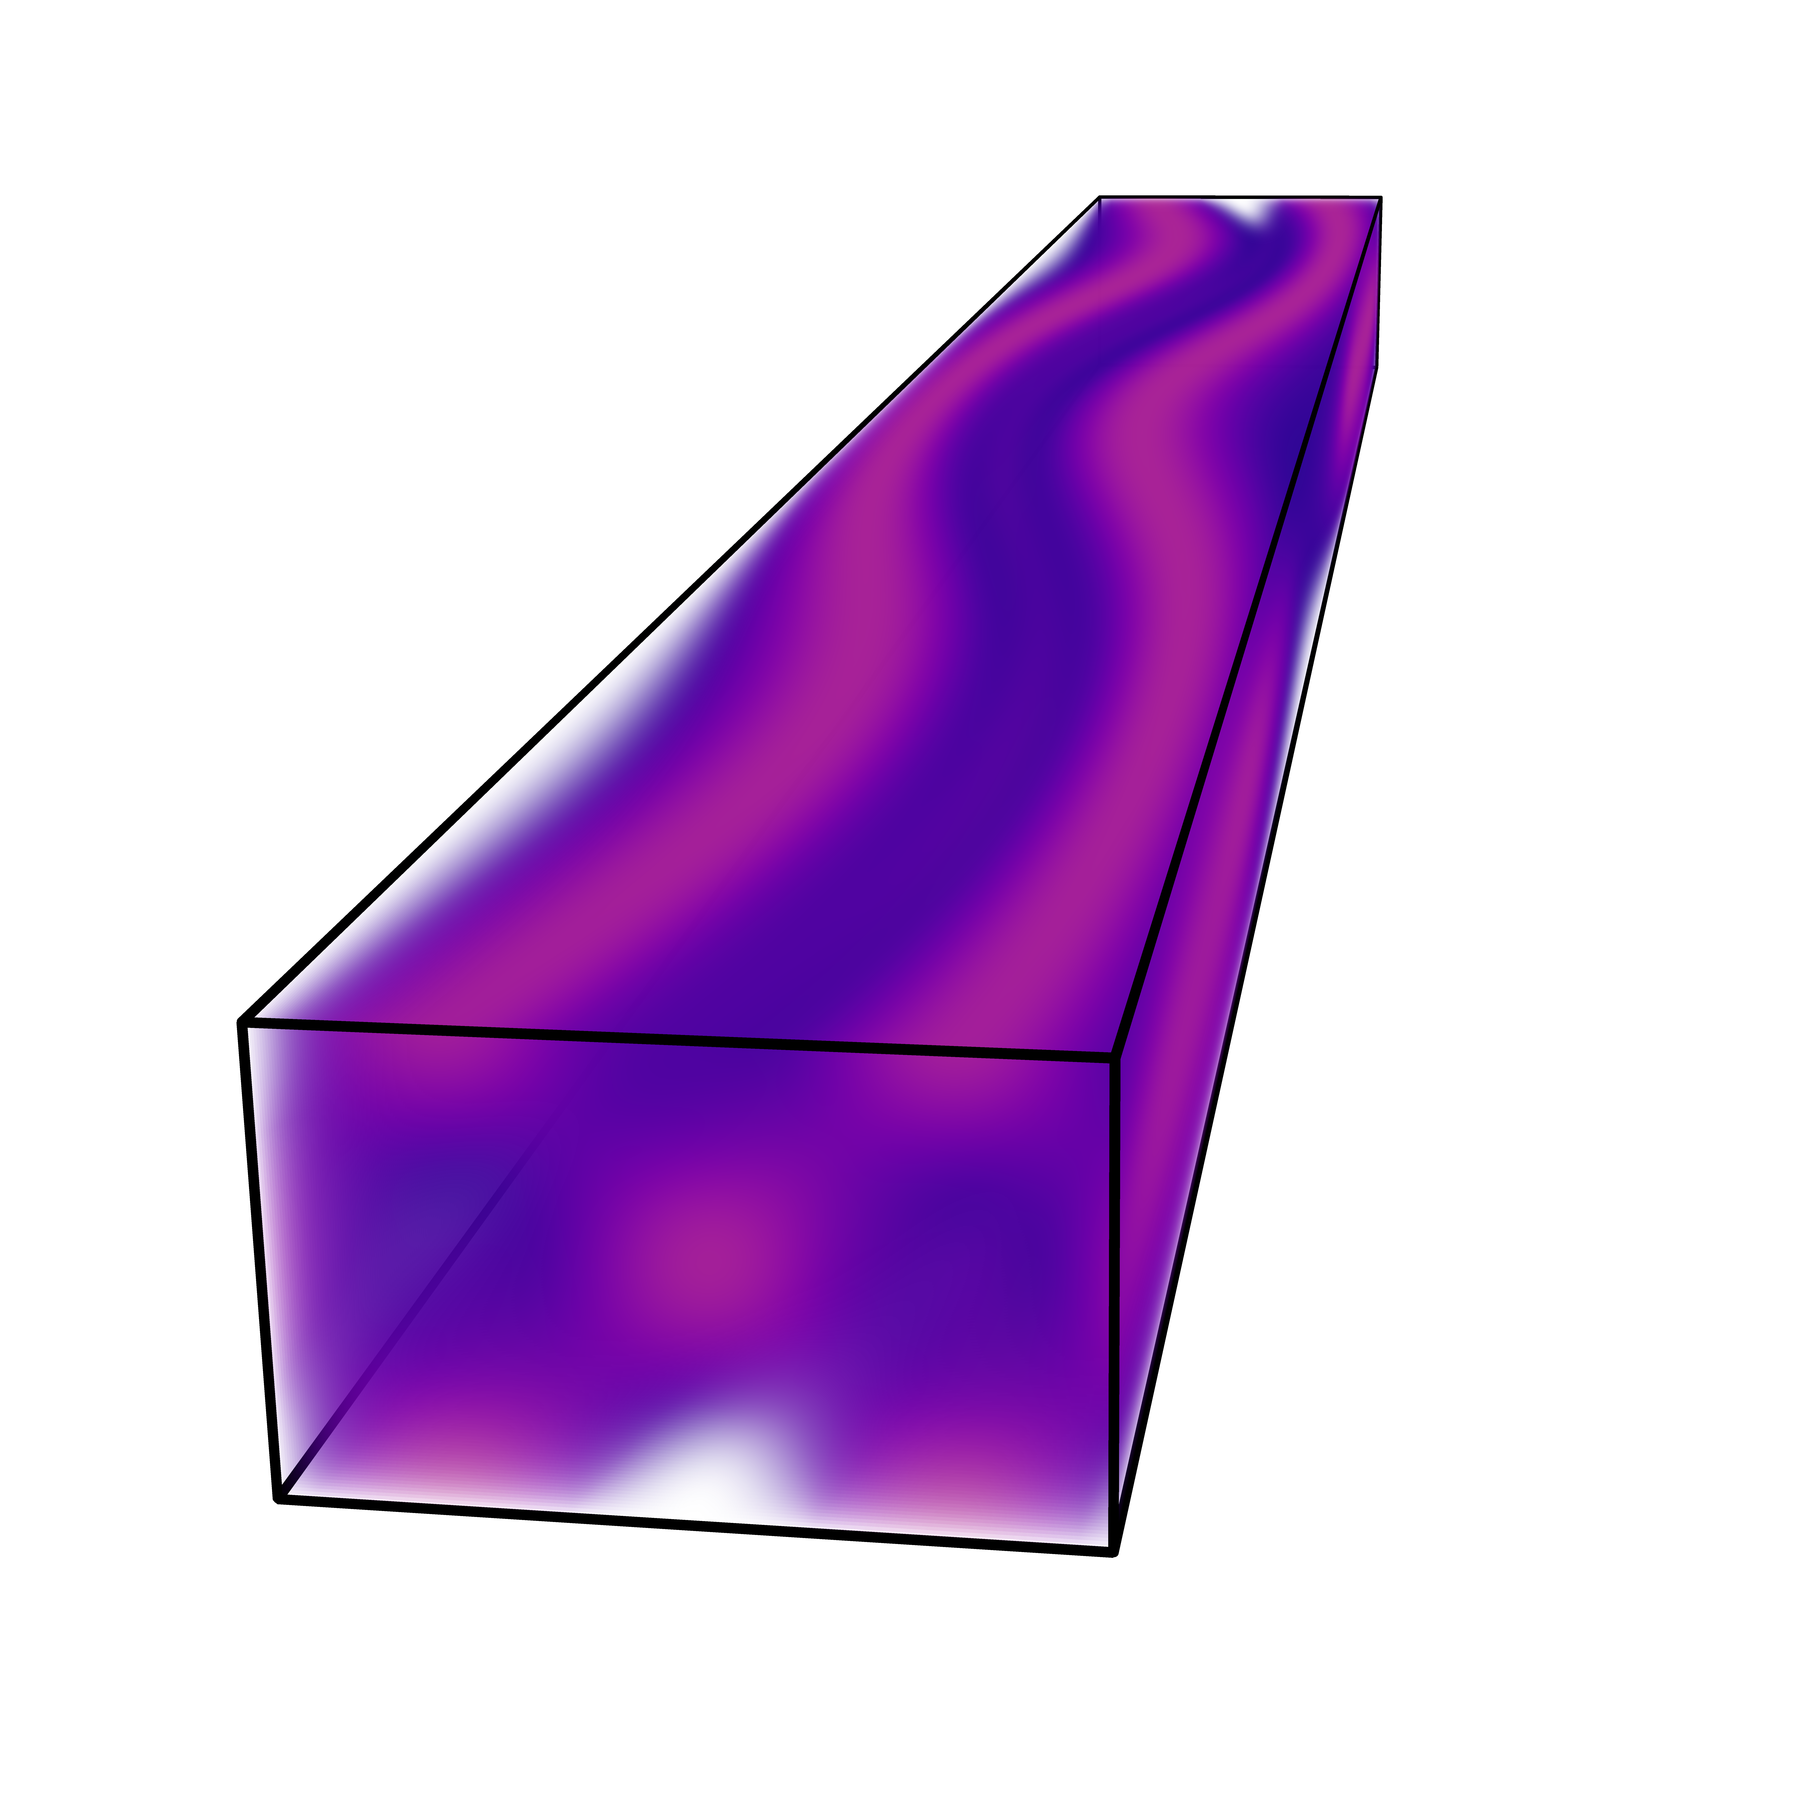
\includegraphics[trim=200 0 350 0, clip=true, width=\textwidth]{Images/dgyre.png}
        \caption{double gyre}
    \end{subfigure}
    \begin{subfigure}{0.33\textwidth}
        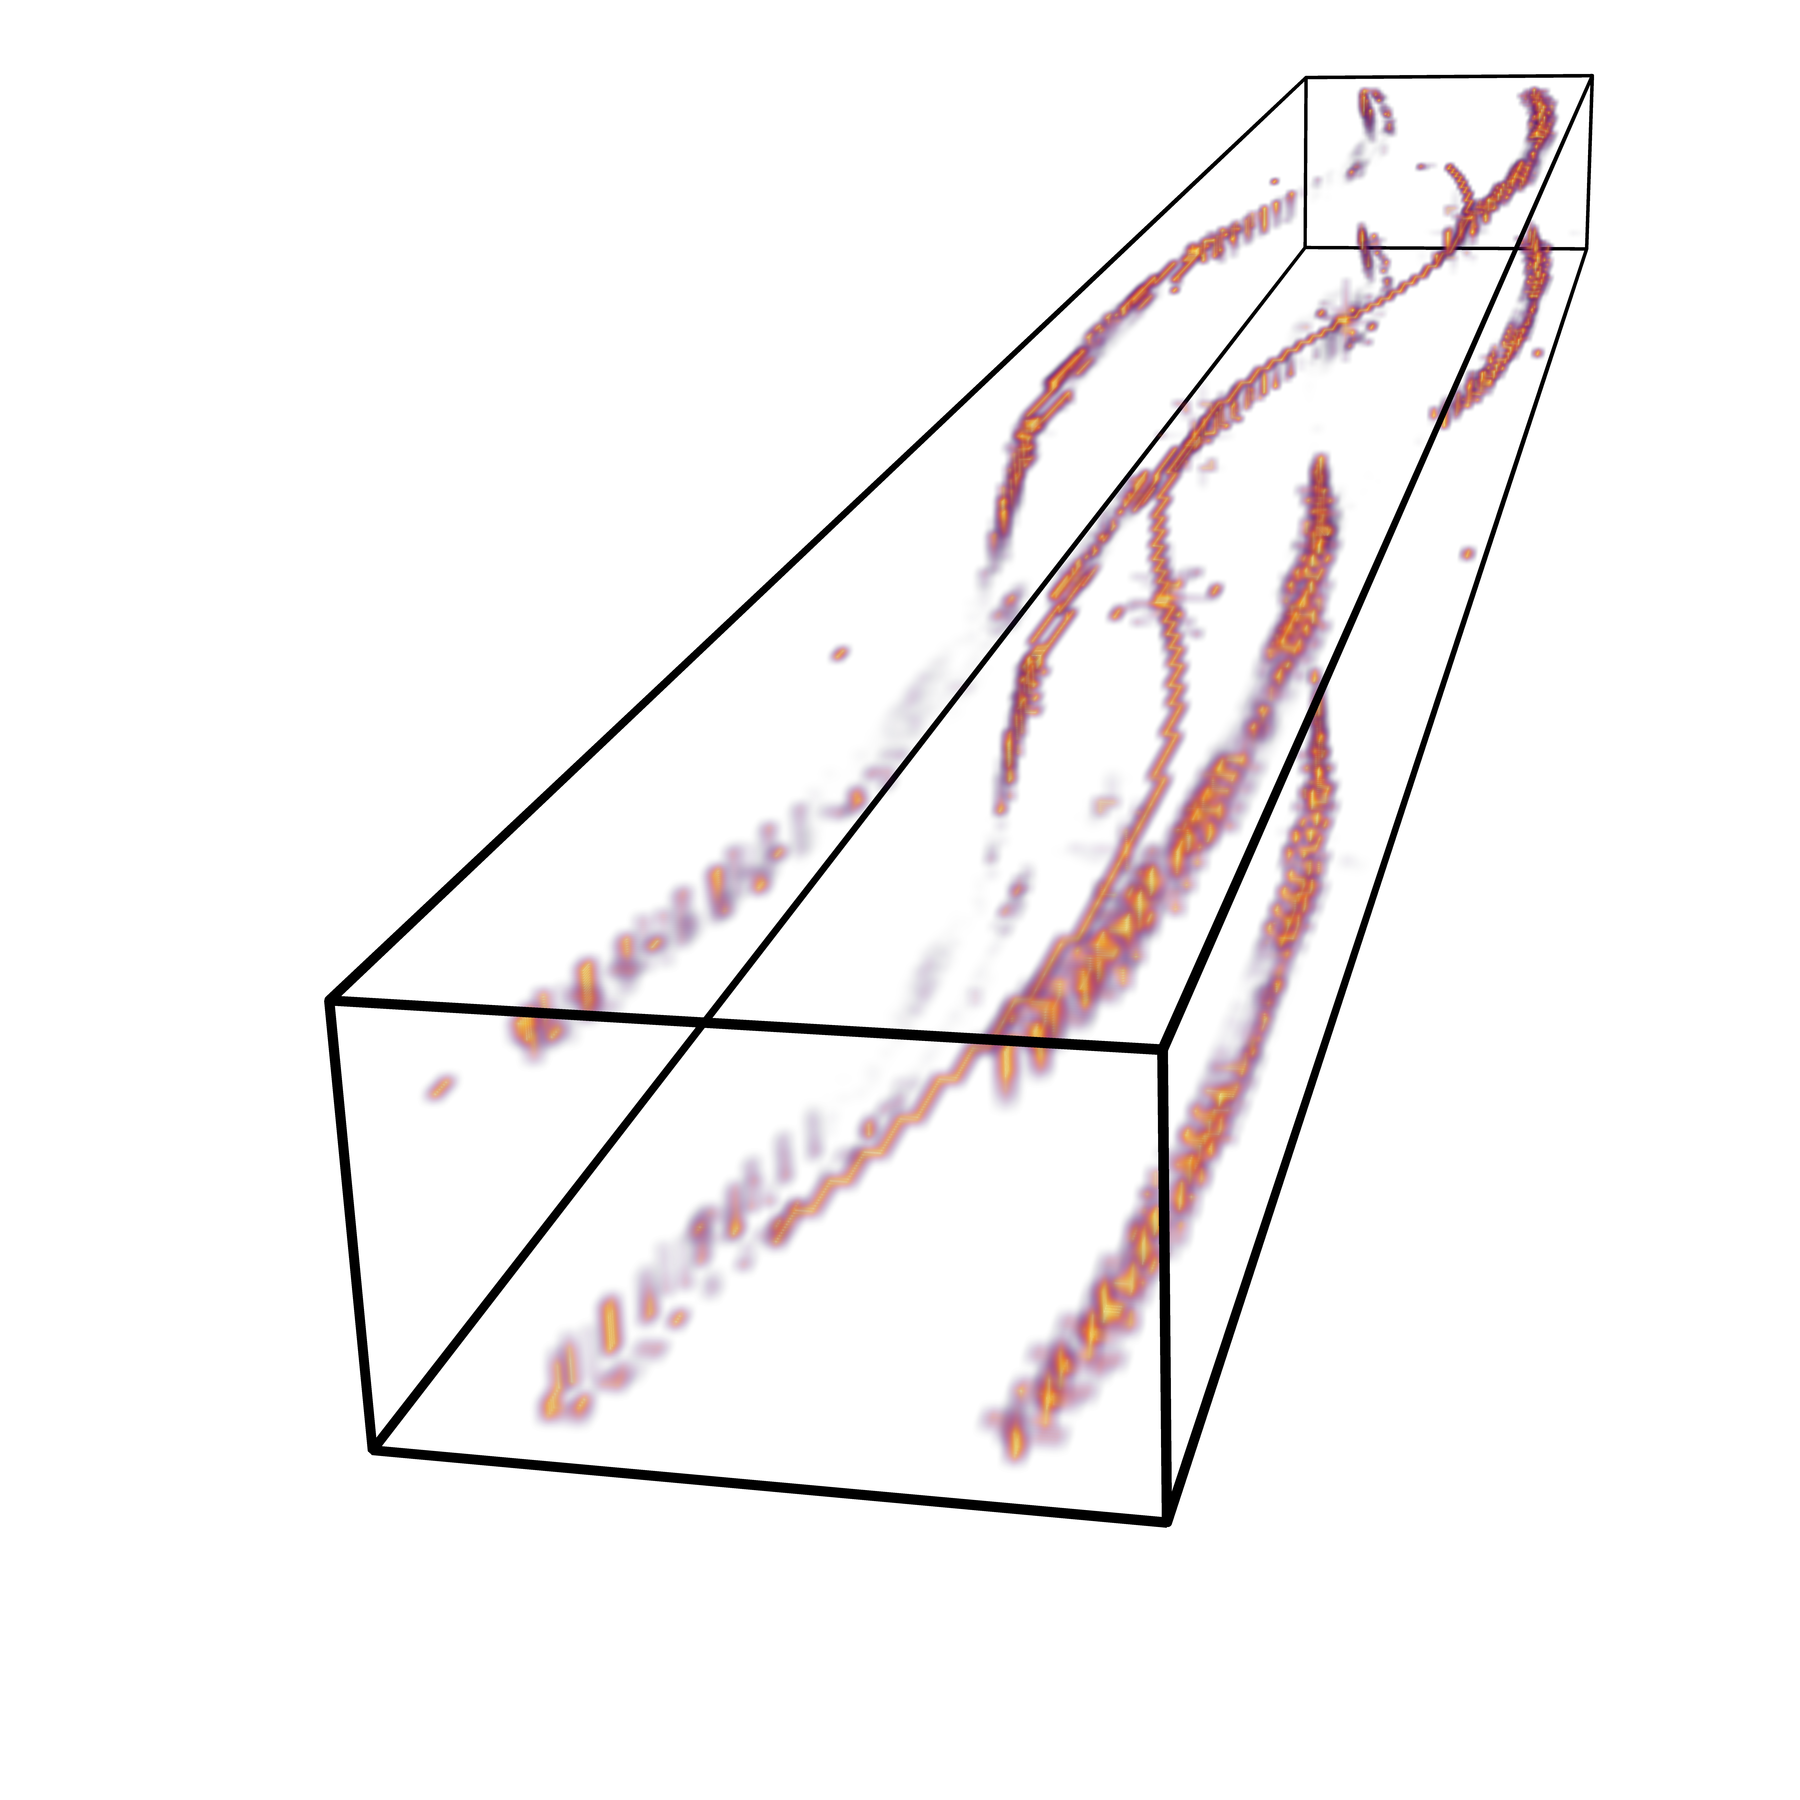
\includegraphics[trim=200 0 200 0, clip=true, width=\textwidth]{Images/RL3D.png}
        \caption{raw lines}
    \end{subfigure}
    \begin{subfigure}{0.33\textwidth}
        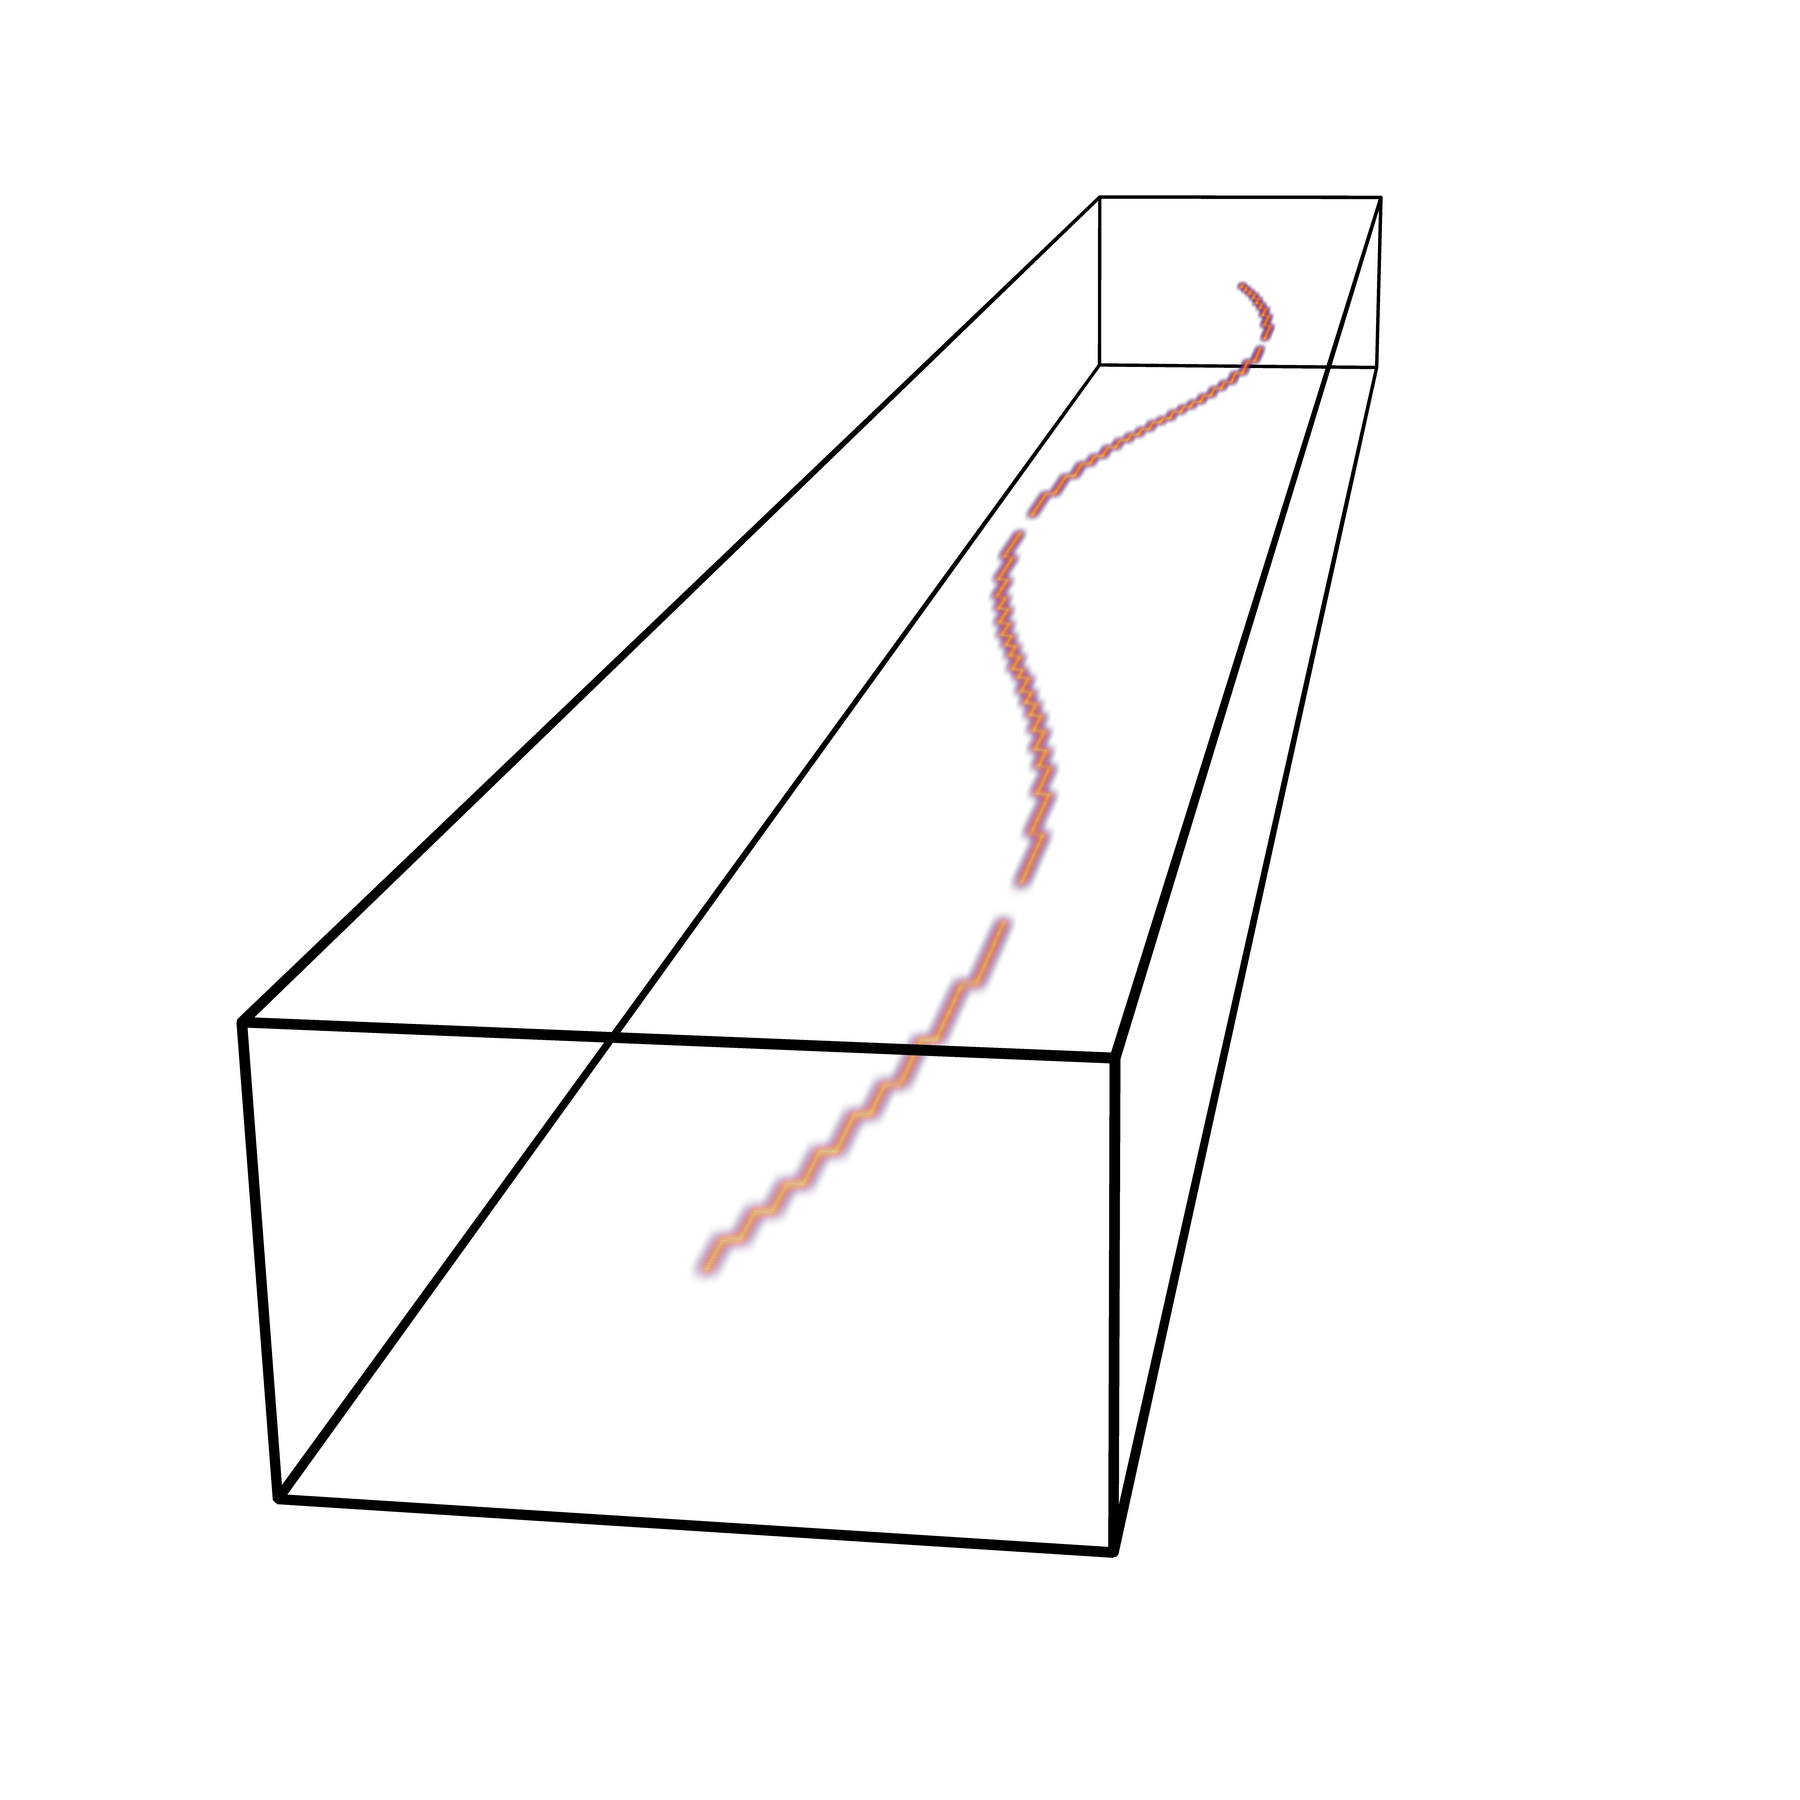
\includegraphics[trim=200 0 200 0, clip=true, width=\textwidth]{Images/RL3Dfilt.png}
        \caption{filtered for $\lambda_2 > 0.7$.}
    \end{subfigure}
    \caption{Uncertain ridge line calculation for double gyre domain.}
\end{figure}